% =====================================================================
%  Chapter 2: Vector Products from Quaternions to Area and Volume
% =====================================================================

\chapter{Vector Products from Quaternions to Area and Volume}
\label{ch:2}
Chapter 1 ended with a problem that sounds innocent: can we multiply vectors?

Numbers multiply easily.  If one number measures a stretch and another measures a
stretch, their product is another stretch.  But vectors carry more information than numbers.
They have length and direction.  A good vector product should somehow remember both.

There is one place where this already works beautifully: the plane.  The secret is to look
at the plane through complex numbers.

\section{Complex numbers as a warm-up}

A vector in the plane can be written as
\[
    (a,b).
\]
A complex number writes the same two pieces of data in a different language:
\[
    a+bi.
\]
At first, the symbol \(i\) may look like a trick.  But geometrically it is one of the most
useful symbols in mathematics.  Multiplying by \(i\) means rotating a plane vector by
\(90^\circ\) counterclockwise.

For example,
\[
    i(3+2i)=3i+2i^2=-2+3i.
\]
So the vector
\[
    (3,2)
\]
has become
\[
    (-2,3).
\]
That is exactly a \(90^\circ\) counterclockwise turn.

\begin{figure}[h]
\centering
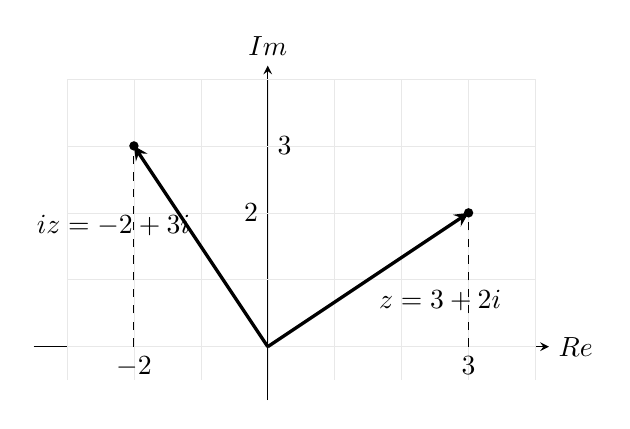
\begin{tikzpicture}[scale=0.85, >=stealth]
    \draw[->] (-3.5,0) -- (4.2,0) node[right] {\(\operatorname{Re}\)};
    \draw[->] (0,-0.8) -- (0,4.2) node[above] {\(\operatorname{Im}\)};

    \draw[step=1, gray!18, very thin] (-3,-0.5) grid (4,4);

    \draw[->, very thick] (0,0) -- (3,2) node[midway, below right] {\(z=3+2i\)};
    \draw[->, very thick] (0,0) -- (-2,3) node[midway, above left] {\(iz=-2+3i\)};

    \draw[dashed] (3,0) -- (3,2);
    \draw[dashed] (-2,0) -- (-2,3);

    \fill (3,2) circle (2pt);
    \fill (-2,3) circle (2pt);

    \node[below] at (3,0) {\(3\)};
    \node[left] at (0,2) {\(2\)};
    \node[below] at (-2,0) {\(-2\)};
    \node[right] at (0,3) {\(3\)};
\end{tikzpicture}
\caption{Multiplication by \(i\) rotates a plane vector by \(90^\circ\).}
\end{figure}

This is the first hint that multiplication can carry geometry.

\subsection{Complex numbers as points and arrows in the plane}

A complex number has the form
\[
    z=a+bi,
\]
where \(a\) and \(b\) are real numbers and
\[
    i^2=-1.
\]

\begin{definition}[Complex numbers]
A \emph{complex number} is an expression
\[
    z=a+bi,
\]
where \(a,b\in\mathbb R\) and \(i^2=-1\).

The number \(a\) is the \emph{real part} of \(z\), and \(b\) is the \emph{imaginary part}
of \(z\):
\[
    \operatorname{Re}(z)=a,\qquad \operatorname{Im}(z)=b.
\]
\end{definition}

We identify
\[
    a+bi
\]
with the point or vector
\[
    (a,b)
\]
in the plane.  So
\[
    3+2i
\]
is the same plane arrow as
\[
    (3,2).
\]

Addition is exactly the vector addition from Chapter 1:
\[
    (a+bi)+(c+di)=(a+c)+(b+d)i.
\]
For example,
\[
    (3+2i)+(-1+4i)=2+6i.
\]
In vector language, this says
\[
    (3,2)+(-1,4)=(2,6).
\]

The length of a complex number is the length of the corresponding vector:
\[
    |a+bi|=\sqrt{a^2+b^2}.
\]
This is the same norm as before, written with complex-number notation.

\begin{example}[A complex number as a vector]
The complex number
\[
    z=-2+5i
\]
corresponds to the vector
\[
    (-2,5).
\]
Its length is
\[
    |z|=\sqrt{(-2)^2+5^2}=\sqrt{29}.
\]
\end{example}

So far, complex numbers have only repackaged plane vectors.  The real surprise comes
from multiplication.

\subsection{Multiplication as scaling and rotation}

To multiply complex numbers, we use ordinary algebra and the rule \(i^2=-1\):
\[
\begin{aligned}
    (a+bi)(c+di)
    &=ac+adi+bci+bdi^2  \\
    &=(ac-bd)+(ad+bc)i.
\end{aligned}
\]

\begin{definition}[Complex multiplication]
For complex numbers
\[
    z=a+bi,\qquad w=c+di,
\]
their product is
\[
    zw=(ac-bd)+(ad+bc)i.
\]
\end{definition}

The formula may look artificial.  It is not.  It is the algebraic shadow of a simple
geometric fact: multiplying complex numbers multiplies lengths and adds angles.

Start with the easiest special case:
\[
    i(a+bi)=ai+bi^2=-b+ai.
\]
So
\[
    a+bi
    \quad\longmapsto\quad
    -b+ai.
\]
In vector notation,
\[
    (a,b)
    \quad\longmapsto\quad
    (-b,a).
\]
That is a \(90^\circ\) counterclockwise rotation.

Multiplying by \(2i\) does two things:
\[
    2i(a+bi)=-2b+2ai.
\]
It rotates by \(90^\circ\) and doubles the length.

\begin{example}[Multiplying by \(1+i\)]
Let
\[
    z=3+i.
\]
Then
\[
    (1+i)z=(1+i)(3+i)=3+i+3i+i^2=2+4i.
\]
The multiplier \(1+i\) has length
\[
    |1+i|=\sqrt2
\]
and direction \(45^\circ\).  So multiplying by \(1+i\) rotates by \(45^\circ\) and
stretches by a factor of \(\sqrt2\).

Indeed,
\[
    |3+i|=\sqrt{10},
\]
while
\[
    |2+4i|=\sqrt{20}=\sqrt2\sqrt{10}.
\]
The length has been multiplied by \(\sqrt2\).
\end{example}

To state the rotation rule clearly, it is useful to write a nonzero complex number in
polar form.  If \(z\neq0\), then
\[
    z=r(\cos\theta+i\sin\theta),
\]
where
\[
    r=|z|
\]
and \(\theta\) is the angle from the positive real axis to the vector \(z\).

\begin{theorem}[Complex multiplication adds angles]
Let
\[
    z=r(\cos\alpha+i\sin\alpha),
    \qquad
    w=s(\cos\beta+i\sin\beta),
\]
where \(r,s>0\).  Then
\[
    zw
    =
    rs\bigl(\cos(\alpha+\beta)+i\sin(\alpha+\beta)\bigr).
\]
So multiplication by \(w\) stretches lengths by \(|w|=s\) and rotates angles by
\(\beta\).
\end{theorem}

\begin{proof}
Multiply:
\[
\begin{aligned}
zw
&=
r(\cos\alpha+i\sin\alpha)\,
s(\cos\beta+i\sin\beta)\\
&=
rs\Bigl(
\cos\alpha\cos\beta
-\sin\alpha\sin\beta
+i(\sin\alpha\cos\beta+\cos\alpha\sin\beta)
\Bigr).
\end{aligned}
\]
Using the angle-addition formulas,
\[
    \cos(\alpha+\beta)
    =
    \cos\alpha\cos\beta-\sin\alpha\sin\beta
\]
and
\[
    \sin(\alpha+\beta)
    =
    \sin\alpha\cos\beta+\cos\alpha\sin\beta,
\]
we get
\[
    zw
    =
    rs\bigl(\cos(\alpha+\beta)+i\sin(\alpha+\beta)\bigr).
\]
\end{proof}

The condition \(r,s>0\) is there for a reason.  The zero complex number has length
\(0\), but it has no direction.  We cannot assign it a unique angle.  Multiplication by
zero does not rotate the plane; it collapses every vector to the origin:
\[
    0\cdot z=0.
\]
So the rotation picture belongs to multiplication by a nonzero complex number.

\subsection{Why two-dimensional geometry has a natural product}

Complex multiplication works because a nonzero plane vector has exactly two pieces of
geometric information:

\[
    \text{length}
    \qquad\text{and}\qquad
    \text{angle}.
\]

Lengths multiply naturally.  Angles add naturally.  That gives a product.

For instance, suppose
\[
    z=2(\cos 30^\circ+i\sin30^\circ)
\]
and
\[
    w=3(\cos 80^\circ+i\sin80^\circ).
\]
Then
\[
    zw
    =
    6(\cos110^\circ+i\sin110^\circ).
\]
The product has length \(6\) and direction \(110^\circ\).

This is a remarkable fact.  The plane is not only a place where vectors live.  It is also a
place where vectors can be multiplied, provided we interpret plane vectors as complex
numbers.

But this product is not the only useful way to combine two plane vectors.

Let
\[
    z=a+bi,\qquad w=c+di.
\]
The complex conjugate of \(z\) is
\[
    \overline z=a-bi.
\]
Now multiply \(\overline z\) and \(w\):
\[
\begin{aligned}
    \overline z\,w
    &=(a-bi)(c+di)\\
    &=ac+adi-bci-bdi^2\\
    &=(ac+bd)+(ad-bc)i.
\end{aligned}
\]
The real part is
\[
    ac+bd.
\]
The imaginary part is
\[
    ad-bc.
\]

Those two expressions are not random.  They are two of the most important measurements
in geometry.

The number
\[
    ac+bd
\]
measures how much the vectors \((a,b)\) and \((c,d)\) point in the same direction.
It will become the \emph{dot product}.

The number
\[
    ad-bc
\]
measures the signed area of the parallelogram made by the two vectors.  It will become
the \(2\times2\) determinant, and later it will reappear as the coefficient of
\[
    dx\wedge dy.
\]

\begin{example}[Two measurements hidden in one complex product]
Let
\[
    z=2+i,\qquad w=4+3i.
\]
Then
\[
    \overline z\,w=(2-i)(4+3i)=8+6i-4i-3i^2=11+2i.
\]
The real part is
\[
    11=2\cdot4+1\cdot3.
\]
The imaginary part is
\[
    2=2\cdot3-1\cdot4.
\]
So the same product has packaged two different geometric measurements:
\[
    \text{directional agreement} \qquad \text{and} \qquad \text{signed area}.
\]
\end{example}

This is the first glimpse of the larger story.  Vector multiplication is not one thing.
Different products measure different geometry.

\subsection{The question Hamilton asked: can triples be multiplied?}

Complex numbers multiply plane vectors.  That raises an irresistible question:

\[
    \text{Can we multiply vectors in space the same way?}
\]

A point in space has three coordinates:
\[
    (x,y,z).
\]
So it is tempting to invent a number of the form
\[
    x+yi+zj
\]
or perhaps
\[
    xi+yj+zk,
\]
and hope that multiplication will behave as cleanly as it does for complex numbers.

The dream is easy to describe.  We would like multiplication to understand three-dimensional
length and rotation.  Multiplying by a special unit should rotate space in some natural way,
just as multiplying by \(i\) rotates the plane.

But there is a problem.  In the plane, there is only one direction perpendicular to the real
axis: the \(i\)-direction.  In space, there are many perpendicular directions.  No single
imaginary unit can control all of them.

Hamilton's breakthrough was to stop trying to multiply triples.  He added one more
component and introduced numbers of the form
\[
    a+bi+cj+dk.
\]
These are called \emph{quaternions}.  They are four-dimensional numbers, but hidden
inside them is exactly the three-dimensional vector geometry we need.

That may sound like a detour.  It is not.  The detour will explain why three-dimensional
vectors have two famous products instead of one: the dot product and the cross product.
Both are already waiting inside quaternion multiplication.

But to see them, we first need to meet the strange multiplication rules for
\[
    i,\qquad j,\qquad k.
\]

\section{Pure imaginary quaternions and three-dimensional vectors}

The complex numbers used one imaginary unit:
\[
    i^2=-1.
\]
For space, Hamilton introduced three:
\[
    i,\qquad j,\qquad k.
\]
They do not behave like ordinary numbers.  That is the whole point.

If they did behave like ordinary commuting numbers, the geometry would break.

\subsection{The units \(i\), \(j\), and \(k\)}

Think of \(i,j,k\) as three perpendicular direction symbols.  For now, they play the roles
of the three standard coordinate directions:
\[
    i \leftrightarrow (1,0,0),\qquad
    j \leftrightarrow (0,1,0),\qquad
    k \leftrightarrow (0,0,1).
\]

A quaternion has the form
\[
    q=a+bi+cj+dk,
\]
where
\[
    a,b,c,d\in\mathbb R.
\]
The number \(a\) is the real part.  The remaining part
\[
    bi+cj+dk
\]
is the imaginary part.

\begin{definition}[Quaternions]
A \emph{quaternion} is an expression
\[
    q=a+bi+cj+dk,
\]
where \(a,b,c,d\in\mathbb R\), and the symbols \(i,j,k\) multiply according to the
quaternion rules stated below.
\end{definition}

For this chapter, the most important quaternions are the ones with no real part.

\begin{definition}[Pure imaginary quaternion]
A quaternion of the form
\[
    bi+cj+dk
\]
is called a \emph{pure imaginary quaternion}.
\end{definition}

Pure imaginary quaternions are the bridge back to ordinary vectors in space:
\[
    bi+cj+dk
    \quad\longleftrightarrow\quad
    (b,c,d).
\]
For example,
\[
    2i-j+3k
    \quad\longleftrightarrow\quad
    (2,-1,3).
\]

Addition and scalar multiplication work exactly as they do for vectors:
\[
    (2i-j+3k)+(i+4j-k)=3i+3j+2k,
\]
and
\[
    5(2i-j+3k)=10i-5j+15k.
\]

So far, this is only a new notation for \(\mathbb R^3\).  Multiplication is where the new
geometry enters.

\subsection{The rule \(i^2=j^2=k^2=ijk=-1\)}

The quaternion units satisfy
\[
    i^2=j^2=k^2=-1
\]
and
\[
    ijk=-1.
\]
These compact rules produce the multiplication table:
\[
\begin{array}{c|ccc}
     & i & j & k \\ \hline
i & -1 & k & -j\\
j & -k & -1 & i\\
k & j & -i & -1
\end{array}
\]

This table says, for example,
\[
    ij=k,
    \qquad
    ji=-k,
\]
and
\[
    jk=i,
    \qquad
    kj=-i,
\]
and
\[
    ki=j,
    \qquad
    ik=-j.
\]

The positive products follow the cyclic order
\[
    i\longrightarrow j\longrightarrow k\longrightarrow i.
\]
Going backward changes the sign.

\begin{figure}[h]
\centering
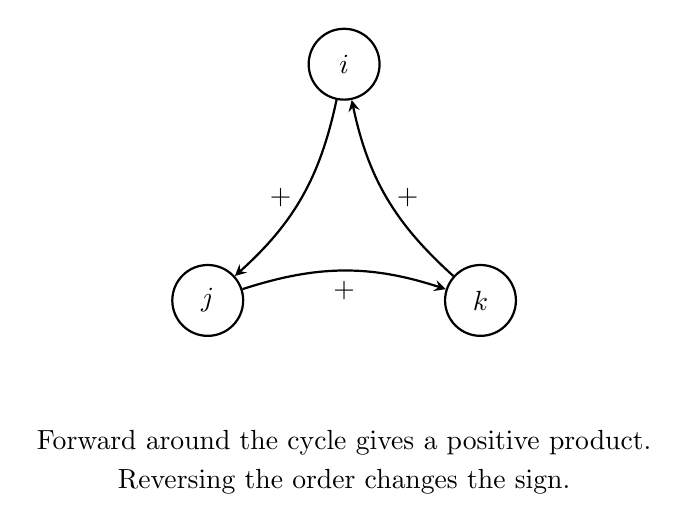
\begin{tikzpicture}[scale=1.0, >=stealth]
    \node[circle, draw, thick, minimum size=9mm] (i) at (90:2) {\(i\)};
    \node[circle, draw, thick, minimum size=9mm] (j) at (210:2) {\(j\)};
    \node[circle, draw, thick, minimum size=9mm] (k) at (330:2) {\(k\)};

    \draw[->, thick] (i) to[bend left=18] node[left] {\(+\)} (j);
    \draw[->, thick] (j) to[bend left=18] node[below] {\(+\)} (k);
    \draw[->, thick] (k) to[bend left=18] node[right] {\(+\)} (i);

    \node at (0,-2.8) {Forward around the cycle gives a positive product.};
    \node at (0,-3.3) {Reversing the order changes the sign.};
\end{tikzpicture}
\caption{The cyclic order \(i\to j\to k\to i\) controls quaternion signs.}
\end{figure}

\begin{example}[Basic products]
Using the table,
\[
    ij=k,
\]
but
\[
    ji=-k.
\]
Also,
\[
    jk=i,
\]
but
\[
    kj=-i.
\]
So multiplication remembers orientation.  The ordered pair \((i,j)\) points toward
\(+k\), while the ordered pair \((j,i)\) points toward \(-k\).
\end{example}

This sign change is not a minor detail.  It is what allows quaternion multiplication to
encode three-dimensional orientation.

\subsection{Noncommutativity: why order matters}

Ordinary real numbers commute:
\[
    ab=ba.
\]
Complex numbers also commute:
\[
    zw=wz.
\]
Quaternions do not.

\[
    ij=k,
    \qquad
    ji=-k.
\]
So
\[
    ij\neq ji.
\]

\begin{definition}[Noncommutative multiplication]
A multiplication rule is called \emph{noncommutative} if changing the order can change
the product:
\[
    ab\neq ba.
\]
Quaternion multiplication is noncommutative.
\end{definition}

The noncommutativity may feel strange, but it is forced by the geometry.

\begin{example}[A commutative attempt breaks]
Suppose we tried to make
\[
    i^2=j^2=k^2=-1,
\]
and also tried to keep multiplication commutative.  If
\[
    ij=k
\]
and
\[
    ji=ij,
\]
then
\[
    k^2=(ij)(ij).
\]
Since multiplication is being assumed commutative in this failed attempt, we could rearrange:
\[
    (ij)(ij)=i^2j^2=(-1)(-1)=1.
\]
So this attempt would force
\[
    k^2=1.
\]
But we wanted
\[
    k^2=-1.
\]
The rules contradict each other.

The lesson is clear: if \(i,j,k\) are going to multiply in a way that matches
three-dimensional orientation, then order has to matter.
\end{example}

Here is a less abstract way to feel the same thing.  In the plane, rotating \(90^\circ\)
and then stretching by \(2\) gives the same final effect as stretching by \(2\) and then
rotating \(90^\circ\).  But in space, rotations around different axes usually do not commute.
Turning a book around one axis and then another can leave it in a different orientation
than doing the same two turns in the opposite order.

Quaternion multiplication has that spatial behavior built into its algebra.

\begin{example}[A product that changes when order changes]
Compute
\[
    (i+j)k
\]
and
\[
    k(i+j).
\]
First,
\[
    (i+j)k=ik+jk.
\]
Using the table,
\[
    ik=-j,\qquad jk=i.
\]
So
\[
    (i+j)k=i-j.
\]
But
\[
    k(i+j)=ki+kj.
\]
Using the table again,
\[
    ki=j,\qquad kj=-i.
\]
Thus
\[
    k(i+j)=j-i.
\]
Therefore
\[
    (i+j)k\neq k(i+j).
\]
In fact,
\[
    k(i+j)=-(i-j).
\]
\end{example}

Order has become geometry.

\subsection{Pure imaginary quaternions as vectors in \(\mathbb R^3\)}

Now return to ordinary vectors.  The vector
\[
    \mathbf v=(x,y,z)
\]
can be written as the pure imaginary quaternion
\[
    V=xi+yj+zk.
\]
This lets us use quaternion multiplication to discover hidden measurements of vectors.

The first surprise comes from squaring a pure imaginary quaternion.

\begin{example}[The square of a pure imaginary quaternion]
Let
\[
    V=2i-j+3k.
\]
Then
\[
\begin{aligned}
    V^2
    &=(2i-j+3k)(2i-j+3k).
\end{aligned}
\]
If we expanded every term, the square terms are
\[
    (2i)^2+(-j)^2+(3k)^2
    =
    4i^2+j^2+9k^2
    =
    -4-1-9
    =
    -14.
\]
The cross terms cancel in pairs.  For instance,
\[
    (2i)(-j)+(-j)(2i)
    =
    -2ij-2ji
    =
    -2k-2(-k)
    =
    0.
\]
The same cancellation happens for the \(i,k\) terms and the \(j,k\) terms.  Therefore
\[
    V^2=-14.
\]

But
\[
    \|(2,-1,3)\|^2=2^2+(-1)^2+3^2=14.
\]
So
\[
    V^2=-\|V\|^2.
\]
\end{example}

This example was not special.

\begin{theorem}[Squaring a pure imaginary quaternion]
Let
\[
    V=xi+yj+zk.
\]
Then
\[
    V^2=-(x^2+y^2+z^2).
\]
Equivalently,
\[
    V^2=-\|V\|^2.
\]
\end{theorem}

\begin{proof}
Expand:
\[
\begin{aligned}
V^2
&=(xi+yj+zk)(xi+yj+zk).
\end{aligned}
\]
The square terms give
\[
    x^2i^2+y^2j^2+z^2k^2
    =
    -x^2-y^2-z^2.
\]
The mixed terms come in opposite pairs:
\[
    xy(ij+ji)=xy(k-k)=0,
\]
\[
    xz(ik+ki)=xz(-j+j)=0,
\]
and
\[
    yz(jk+kj)=yz(i-i)=0.
\]
Thus
\[
    V^2=-(x^2+y^2+z^2).
\]
\end{proof}

This theorem gives a beautiful reason for the minus sign in
\[
    i^2=j^2=k^2=-1.
\]
A pure imaginary quaternion behaves like a direction whose square is negative length
squared.

The zero vector still behaves as expected:
\[
    0i+0j+0k=0,
\]
and
\[
    0^2=0.
\]
Every nonzero pure imaginary quaternion has a negative real square.

\begin{example}[Unit vectors square to \(-1\)]
The coordinate units satisfy
\[
    i^2=j^2=k^2=-1.
\]
But so does any unit direction.

For example, let
\[
    U=\frac{1}{\sqrt3}(i+j+k).
\]
The corresponding vector is
\[
    \left(\frac1{\sqrt3},\frac1{\sqrt3},\frac1{\sqrt3}\right),
\]
which has length \(1\).  By the theorem,
\[
    U^2=-\|U\|^2=-1.
\]
So \(i,j,k\) are not the only square roots of \(-1\) inside the quaternions.  Every unit
direction in space gives one.
\end{example}

This is very different from the complex plane.  In the complex numbers, the two square
roots of \(-1\) are
\[
    i \quad\text{and}\quad -i.
\]
In the quaternions, every unit vector direction gives a square root of \(-1\).  The algebra
has become large enough to hold the geometry of space.

But it has also become stranger.  When we multiply two pure imaginary quaternions, the
answer usually does not stay pure imaginary.

For example,
\[
    ij=k
\]
is pure imaginary.  But
\[
    i^2=-1
\]
is real.  A general product mixes both kinds of output.

Try
\[
    (2i+j)(i+3j).
\]
Then
\[
\begin{aligned}
    (2i+j)(i+3j)
    &=
    2i^2+6ij+ji+3j^2\\
    &=
    2(-1)+6k+(-k)+3(-1)\\
    &=
    -5+5k.
\end{aligned}
\]
The product has a real part,
\[
    -5,
\]
and an imaginary vector part,
\[
    5k.
\]

That split is the doorway to the rest of the chapter.  The real part will become one
kind of vector product.  The imaginary part will become another.  One measures how
much two vectors point together.  The other measures the oriented area they create.
The quaternions do not make us choose between them; they show that both were part of
one multiplication all along.
\section{The scalar and vector parts of a quaternion product}

At the end of the last section, something surprising happened.  When we multiplied two
pure imaginary quaternions, the answer did not usually stay pure imaginary.  It split
into two pieces:
\[
    \text{a real part}
    \qquad\text{and}\qquad
    \text{a pure imaginary vector part}.
\]
That split is not a nuisance.  It is the point.

\subsection{Multiplying two pure imaginary quaternions}

Start with two simple vectors in the plane, but write them as pure imaginary
quaternions:
\[
    U=2i+j,
    \qquad
    V=i+3j.
\]
Their product is
\[
\begin{aligned}
    UV
    &=(2i+j)(i+3j)\\
    &=2i^2+6ij+ji+3j^2\\
    &=-2+6k-k-3\\
    &=-5+5k.
\end{aligned}
\]
The product has two parts:
\[
    -5
    \qquad\text{and}\qquad
    5k.
\]

The real part is
\[
    -5=-(2\cdot 1+1\cdot 3).
\]
The vector part is
\[
    5k=(2\cdot3-1\cdot1)k.
\]

So quaternion multiplication has found two different measurements at once.  The number
\[
    2\cdot1+1\cdot3=5
\]
measures how much the two vectors point together.  The number
\[
    2\cdot3-1\cdot1=5
\]
measures the signed area of the parallelogram they make in the \(xy\)-plane.

\begin{figure}[h]
\centering
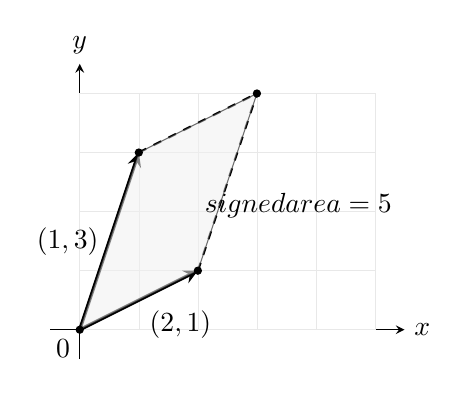
\begin{tikzpicture}[scale=0.75, >=stealth]
    \draw[->] (-0.5,0) -- (5.5,0) node[right] {\(x\)};
    \draw[->] (0,-0.5) -- (0,4.5) node[above] {\(y\)};

    \draw[step=1, gray!18, very thin] (0,0) grid (5,4);

    \coordinate (O) at (0,0);
    \coordinate (U) at (2,1);
    \coordinate (V) at (1,3);
    \coordinate (UV) at (3,4);

    \draw[->, very thick] (O) -- (U) node[midway, below right] {\((2,1)\)};
    \draw[->, very thick] (O) -- (V) node[midway, left] {\((1,3)\)};

    \draw[thick, dashed] (U) -- (UV);
    \draw[thick, dashed] (V) -- (UV);
    \draw[fill=gray!12, opacity=0.55] (O) -- (U) -- (UV) -- (V) -- cycle;

    \fill (O) circle (2pt);
    \fill (U) circle (2pt);
    \fill (V) circle (2pt);
    \fill (UV) circle (2pt);

    \node at (3.7,2.1) {\(\text{signed area}=5\)};
    \node[below left] at (O) {\(0\)};
\end{tikzpicture}
\caption{The vector part \(5k\) records the signed area of the parallelogram.}
\end{figure}

The direction \(k\) matters.  The parallelogram lies in the \(xy\)-plane, so its oriented
area points perpendicular to that plane.  The order \((2,1)\) then \((1,3)\) gives the
positive \(k\)-direction.

If we reverse the order, the real part stays the same, but the vector part changes sign:
\[
\begin{aligned}
    VU
    &=(i+3j)(2i+j)\\
    &=2i^2+ij+6ji+3j^2\\
    &=-2+k-6k-3\\
    &=-5-5k.
\end{aligned}
\]
The same two arrows make the same area, but the opposite orientation.

This is exactly the kind of behavior an oriented area should have.

\subsection{The general product}

Now do the same multiplication without choosing numbers.

Let
\[
    \mathbf u=(u_1,u_2,u_3),
    \qquad
    \mathbf v=(v_1,v_2,v_3),
\]
and write the corresponding pure imaginary quaternions as
\[
    U=u_1i+u_2j+u_3k,
    \qquad
    V=v_1i+v_2j+v_3k.
\]
Expanding \(UV\) gives
\[
\begin{aligned}
UV
&=(u_1i+u_2j+u_3k)(v_1i+v_2j+v_3k)\\
&=u_1v_1i^2+u_1v_2ij+u_1v_3ik\\
&\qquad
 +u_2v_1ji+u_2v_2j^2+u_2v_3jk\\
&\qquad
 +u_3v_1ki+u_3v_2kj+u_3v_3k^2.
\end{aligned}
\]
Using
\[
    i^2=j^2=k^2=-1,
\]
and
\[
    ij=k,\quad jk=i,\quad ki=j,
\]
while reversing order changes the sign, we get
\[
\boxed{
\begin{aligned}
UV
&=-(u_1v_1+u_2v_2+u_3v_3)\\
&\qquad
 +(u_2v_3-u_3v_2)i\\
&\qquad
 +(u_3v_1-u_1v_3)j\\
&\qquad
 +(u_1v_2-u_2v_1)k.
\end{aligned}
}
\]

This formula is long, but it has a simple structure:
\[
    UV
    =
    \text{scalar part}
    +
    \text{vector part}.
\]

\begin{definition}[Scalar part and vector part]
For a quaternion
\[
    q=a+bi+cj+dk,
\]
the \emph{scalar part} is
\[
    \operatorname{Scal}(q)=a,
\]
and the \emph{vector part} is
\[
    \operatorname{Vec}(q)=bi+cj+dk.
\]
\end{definition}

For the product of two pure imaginary quaternions, the scalar part is
\[
    \operatorname{Scal}(UV)=-(u_1v_1+u_2v_2+u_3v_3),
\]
and the vector part is
\[
    \operatorname{Vec}(UV)
    =
    (u_2v_3-u_3v_2)i
    +(u_3v_1-u_1v_3)j
    +(u_1v_2-u_2v_1)k.
\]

The two expressions are important enough to receive their own names.

\begin{definition}[Dot product and cross product from quaternions]
For vectors
\[
    \mathbf u=(u_1,u_2,u_3),
    \qquad
    \mathbf v=(v_1,v_2,v_3),
\]
the \emph{dot product} is
\[
    \mathbf u\cdot\mathbf v
    =
    u_1v_1+u_2v_2+u_3v_3.
\]
The \emph{cross product} is
\[
    \mathbf u\times\mathbf v
    =
    (u_2v_3-u_3v_2)i
    +(u_3v_1-u_1v_3)j
    +(u_1v_2-u_2v_1)k.
\]
\end{definition}

With these names, the quaternion product becomes beautifully short:
\[
\boxed{
    UV= -\mathbf u\cdot\mathbf v+\mathbf u\times\mathbf v.
}
\]

\begin{theorem}[The quaternion product splits into dot and cross]
Let
\[
    U=u_1i+u_2j+u_3k,
    \qquad
    V=v_1i+v_2j+v_3k
\]
be pure imaginary quaternions, corresponding to vectors
\[
    \mathbf u=(u_1,u_2,u_3),
    \qquad
    \mathbf v=(v_1,v_2,v_3).
\]
Then
\[
    UV= -\mathbf u\cdot\mathbf v+\mathbf u\times\mathbf v.
\]
The scalar part of \(UV\) is
\[
    -\mathbf u\cdot\mathbf v,
\]
and the vector part of \(UV\) is
\[
    \mathbf u\times\mathbf v.
\]
\end{theorem}

\begin{proof}
This is exactly the expansion above.  The real terms are
\[
    -u_1v_1-u_2v_2-u_3v_3
    =
    -\mathbf u\cdot\mathbf v.
\]
The \(i\), \(j\), and \(k\) terms are
\[
    (u_2v_3-u_3v_2)i,
\]
\[
    (u_3v_1-u_1v_3)j,
\]
and
\[
    (u_1v_2-u_2v_1)k,
\]
which together form \(\mathbf u\times\mathbf v\).
\end{proof}

The hypothesis that \(U\) and \(V\) are \emph{pure imaginary} matters.  If real parts are
present, new terms appear.

For example, let
\[
    q=1+i,
    \qquad
    r=j.
\]
Then
\[
    qr=(1+i)j=j+ij=j+k.
\]
But if we only used the vector parts \(i\) and \(j\), the formula would give
\[
    -\mathbf i\cdot\mathbf j+\mathbf i\times\mathbf j=k.
\]
It misses the extra \(j\), which came from the real part \(1\) multiplying \(j\).
So the clean split
\[
    UV=-\mathbf u\cdot\mathbf v+\mathbf u\times\mathbf v
\]
belongs to products of pure imaginary quaternions.

\subsection{The scalar part and the dot product}

The scalar part is easiest to feel when two vectors point in the same direction.

Let
\[
    U=3i+4j,
    \qquad
    V=6i+8j.
\]
These represent
\[
    \mathbf u=(3,4,0),
    \qquad
    \mathbf v=(6,8,0).
\]
The second vector is twice the first:
\[
    \mathbf v=2\mathbf u.
\]
Their dot product is
\[
    \mathbf u\cdot\mathbf v
    =
    3\cdot6+4\cdot8+0\cdot0
    =
    18+32
    =
    50.
\]
The scalar part of \(UV\) is therefore
\[
    -50.
\]

The minus sign is not a mistake.  It comes from the fact that
\[
    i^2=j^2=k^2=-1.
\]
When a direction multiplies itself, it contributes a negative real number.

This is why we define
\[
    \mathbf u\cdot\mathbf v
\]
as the \emph{negative} of the scalar part of \(UV\).  The dot product is positive when
vectors point together.

Now compare that with a perpendicular vector:
\[
    W=-4i+3j.
\]
Then
\[
    \mathbf u=(3,4,0),
    \qquad
    \mathbf w=(-4,3,0),
\]
and
\[
    \mathbf u\cdot\mathbf w
    =
    3(-4)+4(3)+0
    =
    -12+12
    =
    0.
\]
So the scalar part of \(UW\) is zero.

The dot product measures directional agreement:
\[
\begin{array}{c|c}
\mathbf u\cdot\mathbf v>0 & \text{the vectors point somewhat together}\\
\mathbf u\cdot\mathbf v=0 & \text{the vectors are perpendicular, if both are nonzero}\\
\mathbf u\cdot\mathbf v<0 & \text{the vectors point somewhat against each other}
\end{array}
\]

\subsection{The vector part and the cross product}

The vector part remembers orientation.

The basic quaternion products give
\[
    ij=k,
    \qquad
    ji=-k.
\]
So
\[
    \mathbf i\times\mathbf j=\mathbf k,
    \qquad
    \mathbf j\times\mathbf i=-\mathbf k.
\]
This is the seed of the right-hand rule.  The ordered pair \(i,j\) points toward \(k\).
Reverse the order, and the direction reverses.

\begin{example}[A three-dimensional product]
Let
\[
    U=2i-j+3k,
    \qquad
    V=i+4j+2k.
\]
The corresponding vectors are
\[
    \mathbf u=(2,-1,3),
    \qquad
    \mathbf v=(1,4,2).
\]
Their dot product is
\[
    \mathbf u\cdot\mathbf v
    =
    2\cdot1+(-1)\cdot4+3\cdot2
    =
    2-4+6
    =
    4.
\]
So the scalar part of \(UV\) is
\[
    -4.
\]

The cross product is
\[
\begin{aligned}
\mathbf u\times\mathbf v
&=
((-1)(2)-3(4))i
+(3(1)-2(2))j
+(2(4)-(-1)(1))k\\
&=
(-2-12)i+(3-4)j+(8+1)k\\
&=
-14i-j+9k.
\end{aligned}
\]
Therefore
\[
    UV=-4-14i-j+9k.
\]
\end{example}

This product has packed two answers into one line:
\[
    \text{directional agreement} \qquad \text{and} \qquad \text{oriented area}.
\]
The dot product is the scalar measurement.  The cross product is the vector measurement.

\subsection{Symmetric and antisymmetric parts of multiplication}

Quaternion multiplication is not commutative:
\[
    UV\neq VU
\]
in general.  But if we add and subtract \(UV\) and \(VU\), the two pieces separate cleanly.

For the example
\[
    U=2i+j,
    \qquad
    V=i+3j,
\]
we found
\[
    UV=-5+5k,
\]
and
\[
    VU=-5-5k.
\]
Adding gives
\[
    UV+VU=-10.
\]
Subtracting gives
\[
    UV-VU=10k.
\]
So
\[
    \frac{UV+VU}{2}=-5,
\]
and
\[
    \frac{UV-VU}{2}=5k.
\]
The average keeps the scalar part.  The half-difference keeps the vector part.

This always happens.

\begin{theorem}[Symmetric and antisymmetric parts]
Let \(U\) and \(V\) be pure imaginary quaternions corresponding to vectors
\(\mathbf u\) and \(\mathbf v\).  Then
\[
    \frac{UV+VU}{2}
    =
    -\mathbf u\cdot\mathbf v,
\]
and
\[
    \frac{UV-VU}{2}
    =
    \mathbf u\times\mathbf v.
\]
\end{theorem}

\begin{proof}
From the product formula,
\[
    UV=-\mathbf u\cdot\mathbf v+\mathbf u\times\mathbf v.
\]
If we reverse the order, the dot product stays the same:
\[
    \mathbf v\cdot\mathbf u=\mathbf u\cdot\mathbf v.
\]
But the cross product changes sign:
\[
    \mathbf v\times\mathbf u=-(\mathbf u\times\mathbf v).
\]
Therefore
\[
    VU=-\mathbf u\cdot\mathbf v-\mathbf u\times\mathbf v.
\]
Adding,
\[
    UV+VU=-2\mathbf u\cdot\mathbf v.
\]
Subtracting,
\[
    UV-VU=2\mathbf u\times\mathbf v.
\]
Dividing by \(2\) gives the result.
\end{proof}

The words \emph{symmetric} and \emph{antisymmetric} describe what happens when we
swap the two inputs.

The dot product is symmetric:
\[
    \mathbf u\cdot\mathbf v=\mathbf v\cdot\mathbf u.
\]
The cross product is antisymmetric:
\[
    \mathbf u\times\mathbf v=-(\mathbf v\times\mathbf u).
\]

This sign change is the same sign change we saw in oriented area:
\[
    \text{area}(\mathbf u,\mathbf v)
    =
    -\text{area}(\mathbf v,\mathbf u).
\]
That idea will return later in a more flexible form as the wedge product.

\subsection{What this explains better than a memorized determinant}

Many calculus books introduce the dot product by a formula and the cross product by
a determinant.  Those formulas are useful, and we will use them.  But by themselves
they can feel like two unrelated tricks.

Quaternion multiplication tells a more coherent story.

Multiplying two pure imaginary quaternions gives
\[
    UV=-\mathbf u\cdot\mathbf v+\mathbf u\times\mathbf v.
\]
One product splits into two geometric measurements.

The scalar part measures how much the two vectors point in the same direction.
The vector part measures the oriented area they create.

That explains why the dot product is symmetric:
\[
    \mathbf u\cdot\mathbf v=\mathbf v\cdot\mathbf u.
\]
Pointing together does not depend on order.

It also explains why the cross product is antisymmetric:
\[
    \mathbf u\times\mathbf v=-(\mathbf v\times\mathbf u).
\]
Oriented area does depend on order.

The dot product deserves its own closer look.  It has no direction, but it controls
length, angle, perpendicularity, projection, and work.  Before following the vector
part into areas and normal directions, we should understand this scalar measurement
well.

\section{The dot product}

The last section pulled the dot product out of the scalar part of quaternion
multiplication:
\[
    \operatorname{Scal}(UV)=-\mathbf u\cdot\mathbf v.
\]
Now we study the dot product on its own.  It is the simplest way to ask a geometric
question:

\[
    \text{How much does one vector point along another?}
\]

\subsection{Algebraic definition and first examples}

Imagine dragging a sled across flat snow.  The sled moves
\[
    \mathbf d=(3,4)
\]
meters: \(3\) meters east and \(4\) meters north.

First suppose the pull is purely east:
\[
    \mathbf F=(10,0).
\]
Only the east part of the motion helps the pull do work.  The northward motion is
sideways to the force.  So the useful multiplication is
\[
    10\cdot3+0\cdot4=30.
\]

Now suppose the force is
\[
    \mathbf F=(6,8).
\]
Then both components help:
\[
    6\cdot3+8\cdot4=18+32=50.
\]

Finally suppose the force is
\[
    \mathbf F=(-4,3).
\]
Then
\[
    (-4)\cdot3+3\cdot4=-12+12=0.
\]
This force is perpendicular to the displacement.  It pulls sideways, so it does no work
along that motion.

The same component-by-component multiplication is the dot product.

\begin{definition}[Dot product]
For vectors in the plane,
\[
    \mathbf u=(u_1,u_2),
    \qquad
    \mathbf v=(v_1,v_2),
\]
the \emph{dot product} is
\[
    \mathbf u\cdot\mathbf v
    =
    u_1v_1+u_2v_2.
\]

For vectors in space,
\[
    \mathbf u=(u_1,u_2,u_3),
    \qquad
    \mathbf v=(v_1,v_2,v_3),
\]
the \emph{dot product} is
\[
    \mathbf u\cdot\mathbf v
    =
    u_1v_1+u_2v_2+u_3v_3.
\]
\end{definition}

\begin{example}[A dot product in space]
Let
\[
    \mathbf u=(2,-1,3),
    \qquad
    \mathbf v=(4,5,-2).
\]
Then
\[
\begin{aligned}
    \mathbf u\cdot\mathbf v
    &=
    2\cdot4+(-1)\cdot5+3\cdot(-2)\\
    &=
    8-5-6\\
    &=
    -3.
\end{aligned}
\]
The negative answer tells us that the two vectors point somewhat against each other.
\end{example}

The dot product behaves like multiplication in several useful ways.

\begin{theorem}[Basic algebra of the dot product]
For vectors \(\mathbf u,\mathbf v,\mathbf w\) and a scalar \(c\),
\[
    \mathbf u\cdot\mathbf v=\mathbf v\cdot\mathbf u,
\]
\[
    \mathbf u\cdot(\mathbf v+\mathbf w)
    =
    \mathbf u\cdot\mathbf v+\mathbf u\cdot\mathbf w,
\]
and
\[
    (c\mathbf u)\cdot\mathbf v
    =
    c(\mathbf u\cdot\mathbf v).
\]
Also,
\[
    \mathbf u\cdot\mathbf u=\|\mathbf u\|^2.
\]
\end{theorem}

\begin{proof}
All four statements follow by writing the components and using ordinary arithmetic.
For example, in space,
\[
\begin{aligned}
\mathbf u\cdot(\mathbf v+\mathbf w)
&=
u_1(v_1+w_1)+u_2(v_2+w_2)+u_3(v_3+w_3)\\
&=
(u_1v_1+u_2v_2+u_3v_3)
+
(u_1w_1+u_2w_2+u_3w_3)\\
&=
\mathbf u\cdot\mathbf v+\mathbf u\cdot\mathbf w.
\end{aligned}
\]
And
\[
    \mathbf u\cdot\mathbf u
    =
    u_1^2+u_2^2+u_3^2
    =
    \|\mathbf u\|^2.
\]
\end{proof}

That last identity is the first sign that the dot product knows about length:
\[
    \|\mathbf u\|=\sqrt{\mathbf u\cdot\mathbf u}.
\]

\subsection{Length, angle, and orthogonality}

The dot product does more than compute a number.  It computes angles.

Take
\[
    \mathbf u=(3,0),
    \qquad
    \mathbf v=(2,2\sqrt3).
\]
Then
\[
    \|\mathbf u\|=3,
\]
and
\[
    \|\mathbf v\|=\sqrt{2^2+(2\sqrt3)^2}=\sqrt{4+12}=4.
\]
Their dot product is
\[
    \mathbf u\cdot\mathbf v
    =
    3\cdot2+0\cdot2\sqrt3
    =
    6.
\]
So
\[
    \frac{\mathbf u\cdot\mathbf v}{\|\mathbf u\|\|\mathbf v\|}
    =
    \frac{6}{3\cdot4}
    =
    \frac12.
\]
The angle whose cosine is \(1/2\) is \(60^\circ\), or \(\pi/3\) radians.  So these vectors
meet at a \(60^\circ\) angle.

\begin{figure}[h]
\centering
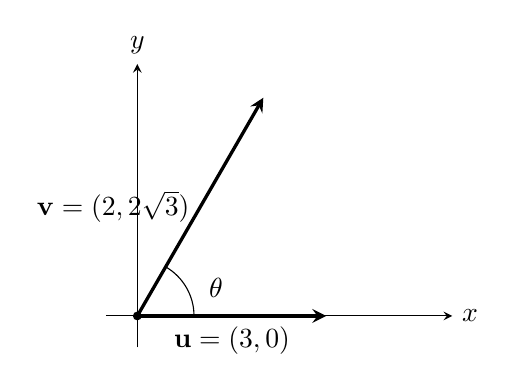
\begin{tikzpicture}[scale=0.8, >=stealth]
    \draw[->] (-0.5,0) -- (5,0) node[right] {\(x\)};
    \draw[->] (0,-0.5) -- (0,4) node[above] {\(y\)};

    \draw[->, very thick] (0,0) -- (3,0) node[midway, below] {\(\mathbf u=(3,0)\)};
    \draw[->, very thick] (0,0) -- (2,3.464) node[midway, left] {\(\mathbf v=(2,2\sqrt3)\)};

    \draw (0.9,0) arc (0:60:0.9);
    \node at (1.25,0.45) {\(\theta\)};

    \fill (0,0) circle (2pt);
\end{tikzpicture}
\caption{The dot product finds the angle through \(\cos\theta\).}
\end{figure}

The pattern is general.

\begin{theorem}[Dot product and angle]
Let \(\mathbf u\) and \(\mathbf v\) be nonzero vectors in the plane or in space.  If
\(\theta\) is the angle between them, with
\[
    0\leq \theta\leq \pi,
\]
then
\[
\boxed{
    \mathbf u\cdot\mathbf v
    =
    \|\mathbf u\|\,\|\mathbf v\|\cos\theta.
}
\]
Equivalently,
\[
    \cos\theta
    =
    \frac{\mathbf u\cdot\mathbf v}{\|\mathbf u\|\,\|\mathbf v\|}.
\]
\end{theorem}

\begin{proof}
Look at the triangle formed by the two vectors \(\mathbf u\), \(\mathbf v\), and
\(\mathbf u-\mathbf v\).  By algebra,
\[
\begin{aligned}
\|\mathbf u-\mathbf v\|^2
&=
(\mathbf u-\mathbf v)\cdot(\mathbf u-\mathbf v)\\
&=
\mathbf u\cdot\mathbf u
-2\mathbf u\cdot\mathbf v
+\mathbf v\cdot\mathbf v\\
&=
\|\mathbf u\|^2+\|\mathbf v\|^2-2\mathbf u\cdot\mathbf v.
\end{aligned}
\]
By the Law of Cosines applied to the same triangle,
\[
    \|\mathbf u-\mathbf v\|^2
    =
    \|\mathbf u\|^2+\|\mathbf v\|^2
    -2\|\mathbf u\|\,\|\mathbf v\|\cos\theta.
\]
Comparing the two formulas gives
\[
    \mathbf u\cdot\mathbf v
    =
    \|\mathbf u\|\,\|\mathbf v\|\cos\theta.
\]
\end{proof}

We required both vectors to be nonzero.  That condition is not cosmetic.  The zero
vector has length \(0\), but it has no direction.  So there is no well-defined angle
between
\[
    \mathbf 0
\]
and
\[
    (1,0,0).
\]
The formula
\[
    \cos\theta
    =
    \frac{\mathbf u\cdot\mathbf v}{\|\mathbf u\|\,\|\mathbf v\|}
\]
would also divide by \(0\).

The dot product still makes sense with the zero vector:
\[
    \mathbf 0\cdot\mathbf v=0.
\]
But the angle interpretation needs two nonzero vectors.

\begin{definition}[Orthogonal vectors]
Two vectors \(\mathbf u\) and \(\mathbf v\) are called \emph{orthogonal} if
\[
    \mathbf u\cdot\mathbf v=0.
\]
When both vectors are nonzero, this means they are perpendicular.
\end{definition}

\begin{example}[A perpendicular pair]
Let
\[
    \mathbf u=(3,4),
    \qquad
    \mathbf v=(-4,3).
\]
Then
\[
    \mathbf u\cdot\mathbf v
    =
    3(-4)+4(3)
    =
    -12+12
    =
    0.
\]
So the two vectors are perpendicular.
\end{example}

There is a useful trick hiding in that example.  In the plane, if
\[
    \mathbf u=(a,b),
\]
then
\[
    (-b,a)
\]
is perpendicular to \(\mathbf u\), because
\[
    (a,b)\cdot(-b,a)
    =
    -ab+ab
    =
    0.
\]
This is the same \(90^\circ\) rotation we saw when multiplying a complex number by
\(i\).

\subsection{Projection onto a line}

The dot product tells us how much one vector lies along another.

Suppose a narrow trail runs in the direction
\[
    \mathbf u=(3,4).
\]
A gust of wind pushes a hiker by the displacement
\[
    \mathbf v=(7,1).
\]
Part of this displacement is along the trail.  Part is sideways.

The dot product finds the along-trail part:
\[
    \mathbf v\cdot\mathbf u
    =
    7\cdot3+1\cdot4
    =
    25.
\]
Also,
\[
    \mathbf u\cdot\mathbf u
    =
    3^2+4^2
    =
    25.
\]
So the coefficient of \(\mathbf u\) in the along-trail part is
\[
    \frac{\mathbf v\cdot\mathbf u}{\mathbf u\cdot\mathbf u}
    =
    \frac{25}{25}
    =
    1.
\]
Thus the projection of \(\mathbf v\) onto the trail direction is
\[
    1\cdot \mathbf u=(3,4).
\]
The sideways leftover is
\[
    \mathbf v-\mathbf u=(7,1)-(3,4)=(4,-3).
\]
Check that it is perpendicular to the trail:
\[
    (4,-3)\cdot(3,4)=12-12=0.
\]

\begin{figure}[h]
\centering
\begin{tikzpicture}[scale=0.75, >=stealth]
    \draw[->] (-0.5,0) -- (8.5,0) node[right] {\(x\)};
    \draw[->] (0,-3.5) -- (0,5.5) node[above] {\(y\)};

    \coordinate (O) at (0,0);
    \coordinate (U) at (3,4);
    \coordinate (V) at (7,1);
    \coordinate (R) at (4,-3);

    \draw[thick, gray!70] (-1,-1.333) -- (4.2,5.6) node[above] {\(\operatorname{span}\{\mathbf u\}\)};

    \draw[->, very thick] (O) -- (V) node[midway, above right] {\(\mathbf v=(7,1)\)};
    \draw[->, very thick] (O) -- (U) node[midway, left] {\(\operatorname{proj}_{\mathbf u}\mathbf v=(3,4)\)};
    \draw[->, thick, dashed] (U) -- (V) node[midway, right] {\((4,-3)\)};

    \draw (2.76, 3.68) -- (3.08, 3.44) -- (3.32, 3.76);

    \fill (O) circle (2pt);
    \fill (U) circle (2pt);
    \fill (V) circle (2pt);
\end{tikzpicture}
\caption{A vector splits into an along-line projection and a perpendicular leftover.}
\end{figure}

\begin{definition}[Projection onto a line]
Let \(\mathbf u\neq \mathbf 0\).  The \emph{projection of \(\mathbf v\) onto the line
spanned by \(\mathbf u\)} is
\[
\boxed{
    \operatorname{proj}_{\mathbf u}\mathbf v
    =
    \frac{\mathbf v\cdot\mathbf u}{\mathbf u\cdot\mathbf u}\,\mathbf u.
}
\]
The scalar component of \(\mathbf v\) in the direction of \(\mathbf u\) is
\[
    \frac{\mathbf v\cdot\mathbf u}{\|\mathbf u\|}.
\]
\end{definition}

The condition
\[
    \mathbf u\neq\mathbf 0
\]
is necessary.  The zero vector does not determine a line direction, and the formula
would divide by
\[
    \mathbf u\cdot\mathbf u=0.
\]
For example, asking for the projection of \((1,2)\) onto the ``direction''
\[
    (0,0)
\]
has no geometric meaning.  There is no direction to project onto.

Projection is not only a formula.  It is a closest approximation.

\begin{theorem}[Projection is the closest vector on the line]
Let \(\mathbf u\neq\mathbf 0\), and let
\[
    \mathbf p=\operatorname{proj}_{\mathbf u}\mathbf v.
\]
Then \(\mathbf p\) is the vector on the line
\[
    \operatorname{span}\{\mathbf u\}
\]
closest to \(\mathbf v\).
\end{theorem}

\begin{proof}
The vector \(\mathbf p\) has the form
\[
    \mathbf p=c\mathbf u,
    \qquad
    c=\frac{\mathbf v\cdot\mathbf u}{\mathbf u\cdot\mathbf u}.
\]
The leftover
\[
    \mathbf r=\mathbf v-\mathbf p
\]
is perpendicular to \(\mathbf u\), because
\[
\begin{aligned}
\mathbf r\cdot\mathbf u
&=
(\mathbf v-c\mathbf u)\cdot\mathbf u\\
&=
\mathbf v\cdot\mathbf u
-
c(\mathbf u\cdot\mathbf u)\\
&=
\mathbf v\cdot\mathbf u
-
\frac{\mathbf v\cdot\mathbf u}{\mathbf u\cdot\mathbf u}
(\mathbf u\cdot\mathbf u)\\
&=0.
\end{aligned}
\]
Now take any other vector \(t\mathbf u\) on the same line.  Then
\[
    \mathbf v-t\mathbf u
    =
    (\mathbf v-\mathbf p)+(\mathbf p-t\mathbf u).
\]
The first vector is perpendicular to the line, and the second vector lies on the line.
So by the Pythagorean theorem,
\[
    \|\mathbf v-t\mathbf u\|^2
    =
    \|\mathbf v-\mathbf p\|^2
    +
    \|\mathbf p-t\mathbf u\|^2.
\]
This is smallest when
\[
    \|\mathbf p-t\mathbf u\|^2=0,
\]
which happens only when
\[
    t\mathbf u=\mathbf p.
\]
\end{proof}

This theorem is the first glimpse of a large idea: dot products allow us to turn geometry
into approximation.  Later, the same idea will become least squares, tangent planes, and
orthogonal projections in higher-dimensional spaces.

\subsection{Work as force times displacement}

In single-variable physics, constant work is often introduced as
\[
    \text{work}=\text{force}\times\text{distance}.
\]
That formula assumes the force points in the same direction as the motion.

The dot product gives the correct formula when force and displacement may point in
different directions.

\begin{definition}[Work by a constant force]
If a constant force \(\mathbf F\) moves an object through displacement \(\mathbf d\),
then the work done by the force is
\[
\boxed{
    W=\mathbf F\cdot\mathbf d.
}
\]
\end{definition}

\begin{example}[Pushing a crate]
A crate moves
\[
    \mathbf d=(4,0)
\]
meters across a floor.  A force
\[
    \mathbf F=(12,5)
\]
newtons acts on it.  The work done is
\[
    W=\mathbf F\cdot\mathbf d
    =
    12\cdot4+5\cdot0
    =
    48.
\]
So the force does
\[
    48\ \text{joules}
\]
of work.

The vertical component \(5\) does not contribute to the work across the floor, because
the displacement has no vertical component.
\end{example}

Using the angle formula for the dot product,
\[
    \mathbf F\cdot\mathbf d
    =
    \|\mathbf F\|\,\|\mathbf d\|\cos\theta.
\]
So only the component of the force in the direction of motion contributes to the work.

If the force is perpendicular to the displacement, then
\[
    \theta=\frac{\pi}{2},
    \qquad
    \cos\theta=0,
\]
and the work is zero.

If the force points against the displacement, then
\[
    \cos\theta<0,
\]
and the work is negative.  This is what friction does.

\subsection{Cauchy--Schwarz and the geometry of approximation}

A projection cannot be longer than the vector being projected.

For instance, if \(\widehat{\mathbf u}\) is a unit vector, then
\[
    \mathbf v\cdot\widehat{\mathbf u}
\]
is the signed length of the shadow of \(\mathbf v\) in the direction
\(\widehat{\mathbf u}\).  A shadow on a line cannot be longer than the object casting
it:
\[
    |\mathbf v\cdot\widehat{\mathbf u}|
    \leq
    \|\mathbf v\|.
\]
If \(\mathbf u\) is not a unit vector, the same idea becomes
\[
    |\mathbf u\cdot\mathbf v|
    \leq
    \|\mathbf u\|\,\|\mathbf v\|.
\]

\begin{theorem}[Cauchy--Schwarz inequality]
For vectors \(\mathbf u\) and \(\mathbf v\) in the plane or in space,
\[
\boxed{
    |\mathbf u\cdot\mathbf v|
    \leq
    \|\mathbf u\|\,\|\mathbf v\|.
}
\]
If both vectors are nonzero, equality holds exactly when the two vectors lie on the same
line through the origin.
\end{theorem}

\begin{proof}
If either vector is zero, then both sides are \(0\), so the inequality is true.

Now suppose both vectors are nonzero.  Let \(\theta\) be the angle between them.
Using the angle formula,
\[
    \mathbf u\cdot\mathbf v
    =
    \|\mathbf u\|\,\|\mathbf v\|\cos\theta.
\]
Taking absolute values,
\[
    |\mathbf u\cdot\mathbf v|
    =
    \|\mathbf u\|\,\|\mathbf v\|\,|\cos\theta|.
\]
Since
\[
    |\cos\theta|\leq 1,
\]
we get
\[
    |\mathbf u\cdot\mathbf v|
    \leq
    \|\mathbf u\|\,\|\mathbf v\|.
\]
Equality holds when
\[
    |\cos\theta|=1,
\]
which means
\[
    \theta=0
    \quad\text{or}\quad
    \theta=\pi.
\]
So the vectors point in the same direction or in opposite directions.  Either way, they
lie on the same line through the origin.
\end{proof}

The equality condition needs the nonzero assumption.  If
\[
    \mathbf u=\mathbf 0,
\]
then
\[
    |\mathbf u\cdot\mathbf v|=0
    =
    \|\mathbf u\|\,\|\mathbf v\|
\]
for every \(\mathbf v\).  Equality holds, but not because the zero vector has the same
or opposite direction as \(\mathbf v\).  The zero vector has no direction.

Cauchy--Schwarz says that the dot product cannot be too large.  It is the algebraic
version of a geometric fact: the shadow of a vector cannot exceed the vector itself.

It also explains why the angle formula is safe:
\[
    \cos\theta
    =
    \frac{\mathbf u\cdot\mathbf v}{\|\mathbf u\|\|\mathbf v\|}.
\]
Cauchy--Schwarz guarantees that the right side lies between \(-1\) and \(1\), exactly
where a cosine should live.

The dot product measures agreement, projection, and work.  But the quaternion
product had another half.  The vector part does not measure agreement; it measures
oriented area.  It points perpendicular to the plane of two vectors, and its length is the
area of their parallelogram.  That object is the cross product, and it is stranger than
the dot product in one important way: it only works in three-dimensional space.
\section{The cross product}

The dot product measured agreement:
\[
    \mathbf u\cdot\mathbf v
    =
    \|\mathbf u\|\,\|\mathbf v\|\cos\theta.
\]
It told us how much one vector points along another.  But the quaternion product had
another half:
\[
    UV=-\mathbf u\cdot\mathbf v+\mathbf u\times\mathbf v.
\]
The vector part is the cross product.  It does not measure agreement.  It measures
oriented area.

\subsection{A first cross product}

Picture a small rectangular metal plate lying flat on a workbench.  One edge points
\(2\) units in the \(x\)-direction, and the adjacent edge points \(3\) units in the
\(y\)-direction:
\[
    \mathbf u=2\mathbf i,
    \qquad
    \mathbf v=3\mathbf j.
\]
The area of the rectangle is
\[
    2\cdot 3=6.
\]
But the rectangle also has an orientation.  If we walk first along \(\mathbf u\) and then
along \(\mathbf v\), the right-hand rule points upward, in the \(\mathbf k\)-direction.

The cross product records both pieces:
\[
    \mathbf u\times\mathbf v
    =
    (2\mathbf i)\times(3\mathbf j)
    =
    6\mathbf k.
\]
Its length is the area:
\[
    \|\mathbf u\times\mathbf v\|=6.
\]
Its direction is perpendicular to the plate.

If we reverse the order, the same plate gets the opposite orientation:
\[
    \mathbf v\times\mathbf u
    =
    (3\mathbf j)\times(2\mathbf i)
    =
    -6\mathbf k.
\]
The area is still \(6\), but the sign has flipped.

\begin{figure}[h]
\centering
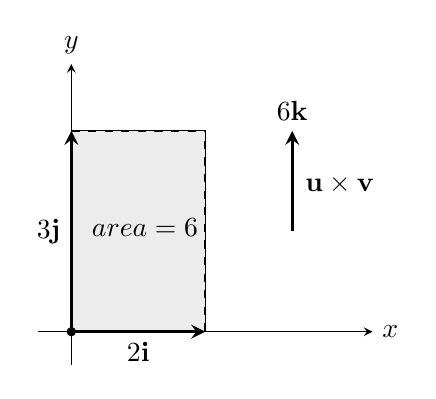
\begin{tikzpicture}[scale=0.85, >=stealth]
    \draw[->] (-0.5,0) -- (4.5,0) node[right] {\(x\)};
    \draw[->] (0,-0.5) -- (0,4) node[above] {\(y\)};

    \coordinate (O) at (0,0);
    \coordinate (U) at (2,0);
    \coordinate (V) at (0,3);
    \coordinate (UV) at (2,3);

    \draw[fill=gray!15] (O) -- (U) -- (UV) -- (V) -- cycle;

    \draw[->, very thick] (O) -- (U) node[midway, below] {\(2\mathbf i\)};
    \draw[->, very thick] (O) -- (V) node[midway, left] {\(3\mathbf j\)};
    \draw[thick, dashed] (U) -- (UV);
    \draw[thick, dashed] (V) -- (UV);

    \node at (1.1,1.55) {\(\text{area}=6\)};

    \draw[->, very thick] (3.3,1.5) -- (3.3,3.0) node[above] {\(6\mathbf k\)};
    \node[right] at (3.35,2.2) {\(\mathbf u\times\mathbf v\)};

    \fill (O) circle (2pt);
\end{tikzpicture}
\caption{The cross product points perpendicular to the oriented rectangle.}
\end{figure}

This first example already shows the main idea:

\[
    \mathbf u\times\mathbf v
    =
    \text{oriented area vector}.
\]

\subsection{Algebraic definition and the right-hand rule}

The cross product is defined only for vectors in three-dimensional space.  If
\[
    \mathbf u=(u_1,u_2,u_3),
    \qquad
    \mathbf v=(v_1,v_2,v_3),
\]
then
\[
\boxed{
\begin{aligned}
\mathbf u\times\mathbf v
&=
(u_2v_3-u_3v_2)\mathbf i\\
&\qquad
+(u_3v_1-u_1v_3)\mathbf j\\
&\qquad
+(u_1v_2-u_2v_1)\mathbf k.
\end{aligned}
}
\]

This is exactly the vector part of the quaternion product from \(\S 2.3\).

The basic products are
\[
    \mathbf i\times\mathbf j=\mathbf k,
    \qquad
    \mathbf j\times\mathbf k=\mathbf i,
    \qquad
    \mathbf k\times\mathbf i=\mathbf j.
\]
These follow the cyclic order
\[
    \mathbf i\to \mathbf j\to \mathbf k\to \mathbf i.
\]
Reversing the order changes the sign:
\[
    \mathbf j\times\mathbf i=-\mathbf k,
    \qquad
    \mathbf k\times\mathbf j=-\mathbf i,
    \qquad
    \mathbf i\times\mathbf k=-\mathbf j.
\]

\begin{figure}[h]
\centering
\begin{tikzpicture}[scale=1.0, >=stealth]
    \draw[->, thick] (0,0) -- (2.4,0) node[right] {\(\mathbf i\)};
    \draw[->, thick] (0,0) -- (0,2.4) node[above] {\(\mathbf j\)};
    \draw[->, thick] (0,0) -- (-1.4,-1.4) node[below left] {\(\mathbf k\)};

    \draw[->] (0.75,0.15) arc (10:80:0.8);
    \node at (1.1,0.85) {\(\mathbf i\to\mathbf j\)};

    \node[right] at (2.7,1.4) {\(\mathbf i\times\mathbf j=\mathbf k\)};
    \node[right] at (2.7,0.8) {\(\mathbf j\times\mathbf i=-\mathbf k\)};
\end{tikzpicture}
\caption{The right-hand rule is the orientation rule for the cross product.}
\end{figure}

Here is a full computation.

\begin{example}[A cross product in space]
Let
\[
    \mathbf u=(2,-1,3),
    \qquad
    \mathbf v=(1,4,2).
\]
Then
\[
\begin{aligned}
\mathbf u\times\mathbf v
&=
((-1)(2)-3(4))\mathbf i\\
&\qquad
+(3(1)-2(2))\mathbf j\\
&\qquad
+(2(4)-(-1)(1))\mathbf k\\
&=
(-2-12)\mathbf i+(3-4)\mathbf j+(8+1)\mathbf k\\
&=
-14\mathbf i-\mathbf j+9\mathbf k.
\end{aligned}
\]
So
\[
    (2,-1,3)\times(1,4,2)=(-14,-1,9).
\]
\end{example}

The formula is not beautiful by itself.  The geometry makes it worth remembering.

\subsection{The cross product is perpendicular to both inputs}

Take
\[
    \mathbf u=(2,-1,3),
    \qquad
    \mathbf v=(1,4,2),
\]
from the previous example.  We found
\[
    \mathbf u\times\mathbf v=(-14,-1,9).
\]
Now dot this result with \(\mathbf u\):
\[
\begin{aligned}
    \mathbf u\cdot(\mathbf u\times\mathbf v)
    &=
    (2,-1,3)\cdot(-14,-1,9)\\
    &=
    2(-14)+(-1)(-1)+3(9)\\
    &=
    -28+1+27\\
    &=0.
\end{aligned}
\]
So \(\mathbf u\times\mathbf v\) is perpendicular to \(\mathbf u\).

Dot it with \(\mathbf v\):
\[
\begin{aligned}
    \mathbf v\cdot(\mathbf u\times\mathbf v)
    &=
    (1,4,2)\cdot(-14,-1,9)\\
    &=
    -14-4+18\\
    &=0.
\end{aligned}
\]
So it is also perpendicular to \(\mathbf v\).

\begin{theorem}[Basic algebra of the cross product]
For vectors \(\mathbf u,\mathbf v,\mathbf w\in\mathbb R^3\) and a scalar \(c\),
\[
    \mathbf u\times\mathbf v=-(\mathbf v\times\mathbf u),
\]
\[
    \mathbf u\times(\mathbf v+\mathbf w)
    =
    \mathbf u\times\mathbf v+\mathbf u\times\mathbf w,
\]
\[
    (c\mathbf u)\times\mathbf v
    =
    c(\mathbf u\times\mathbf v),
\]
and
\[
    \mathbf u\times\mathbf u=\mathbf 0.
\]
Also,
\[
    \mathbf u\cdot(\mathbf u\times\mathbf v)=0,
    \qquad
    \mathbf v\cdot(\mathbf u\times\mathbf v)=0.
\]
Thus \(\mathbf u\times\mathbf v\) is perpendicular to both \(\mathbf u\) and
\(\mathbf v\).
\end{theorem}

\begin{proof}
The first four identities follow by substituting components into the formula for the
cross product and simplifying.

For perpendicularity, write
\[
\mathbf u\times\mathbf v
=
(u_2v_3-u_3v_2,\,
u_3v_1-u_1v_3,\,
u_1v_2-u_2v_1).
\]
Then
\[
\begin{aligned}
\mathbf u\cdot(\mathbf u\times\mathbf v)
&=
u_1(u_2v_3-u_3v_2)
+u_2(u_3v_1-u_1v_3)
+u_3(u_1v_2-u_2v_1)\\
&=
u_1u_2v_3-u_1u_3v_2
+u_2u_3v_1-u_1u_2v_3
+u_1u_3v_2-u_2u_3v_1\\
&=0.
\end{aligned}
\]
The proof that
\[
    \mathbf v\cdot(\mathbf u\times\mathbf v)=0
\]
is the same cancellation with the roles arranged differently.
\end{proof}

The identity
\[
    \mathbf u\times\mathbf v=-(\mathbf v\times\mathbf u)
\]
is worth pausing over.  The cross product is not commutative.  This is not a defect.
It is exactly what oriented area demands.

For example,
\[
    \mathbf i\times\mathbf j=\mathbf k,
\]
but
\[
    \mathbf j\times\mathbf i=-\mathbf k.
\]
The two ordered pairs make the same parallelogram, but with opposite orientation.

\subsection{Cross product as oriented area}

A tilted parallelogram has area
\[
    \text{base}\times\text{height}.
\]
If two vectors \(\mathbf u\) and \(\mathbf v\) meet at angle \(\theta\), then the base is
\[
    \|\mathbf u\|,
\]
and the height is
\[
    \|\mathbf v\|\sin\theta.
\]
So the area is
\[
    \|\mathbf u\|\,\|\mathbf v\|\sin\theta.
\]

The cross product has exactly this length.

\begin{example}[Area of a slanted parallelogram]
Let
\[
    \mathbf u=(3,0,0),
    \qquad
    \mathbf v=(1,2,0).
\]
These vectors lie in the \(xy\)-plane.  Their cross product is
\[
\begin{aligned}
\mathbf u\times\mathbf v
&=
(3\mathbf i)\times(\mathbf i+2\mathbf j)\\
&=
3(\mathbf i\times\mathbf i)+6(\mathbf i\times\mathbf j)\\
&=
0+6\mathbf k\\
&=
6\mathbf k.
\end{aligned}
\]
The parallelogram has base \(3\) and height \(2\), so its area is \(6\).  The cross
product says the same thing:
\[
    \|\mathbf u\times\mathbf v\|=6.
\]
The positive \(\mathbf k\)-direction records that the ordered pair
\[
    \mathbf u,\mathbf v
\]
turns counterclockwise in the \(xy\)-plane.
\end{example}

\begin{theorem}[Length of the cross product]
Let \(\mathbf u\) and \(\mathbf v\) be nonzero vectors in \(\mathbb R^3\), and let
\(\theta\) be the angle between them, with
\[
    0\leq \theta\leq \pi.
\]
Then
\[
\boxed{
    \|\mathbf u\times\mathbf v\|
    =
    \|\mathbf u\|\,\|\mathbf v\|\sin\theta.
}
\]
Therefore \(\|\mathbf u\times\mathbf v\|\) is the area of the parallelogram spanned by
\(\mathbf u\) and \(\mathbf v\).
\end{theorem}

\begin{proof}
A direct component calculation gives the identity
\[
    \|\mathbf u\times\mathbf v\|^2
    =
    \|\mathbf u\|^2\|\mathbf v\|^2-(\mathbf u\cdot\mathbf v)^2.
\]
Using the dot product formula
\[
    \mathbf u\cdot\mathbf v
    =
    \|\mathbf u\|\,\|\mathbf v\|\cos\theta,
\]
we get
\[
\begin{aligned}
\|\mathbf u\times\mathbf v\|^2
&=
\|\mathbf u\|^2\|\mathbf v\|^2
-
\|\mathbf u\|^2\|\mathbf v\|^2\cos^2\theta\\
&=
\|\mathbf u\|^2\|\mathbf v\|^2(1-\cos^2\theta)\\
&=
\|\mathbf u\|^2\|\mathbf v\|^2\sin^2\theta.
\end{aligned}
\]
Since \(0\leq \theta\leq \pi\), we have \(\sin\theta\geq0\).  Taking square roots gives
\[
    \|\mathbf u\times\mathbf v\|
    =
    \|\mathbf u\|\,\|\mathbf v\|\sin\theta.
\]
\end{proof}

The nonzero condition is needed for the angle \(\theta\).  The zero vector has no
direction, so there is no well-defined angle between
\[
    \mathbf 0
\]
and
\[
    (1,0,0).
\]
The cross product itself still makes sense:
\[
    \mathbf 0\times(1,0,0)=\mathbf 0.
\]
The area of the collapsed parallelogram is \(0\).  But the angle formula should not be
used with a zero vector.

There is another warning.  The cross product gives a \emph{direction} only when the
parallelogram has positive area.  If
\[
    \mathbf u=(1,0,0),
    \qquad
    \mathbf v=(2,0,0),
\]
then the two vectors are parallel, and
\[
    \mathbf u\times\mathbf v=\mathbf 0.
\]
The parallelogram has collapsed to a line segment.  It has no preferred normal
direction.  So the zero cross product is not pointing in some mysterious direction.  It is
telling us that there is no oriented area vector to point anywhere.

\subsection{Normal vectors to planes}

A plane can be described by directions lying inside it, or by a vector perpendicular to
it.  The cross product turns the first description into the second.

Suppose a wooden sign is supported by a flat metal plate.  The plate passes through
the point
\[
    P=(1,0,2)
\]
and contains the two direction vectors
\[
    \mathbf a=(2,1,0),
    \qquad
    \mathbf b=(0,1,3).
\]
A vector perpendicular to the plate is
\[
\begin{aligned}
\mathbf n
&=
\mathbf a\times\mathbf b\\
&=
(2,1,0)\times(0,1,3)\\
&=
(1\cdot3-0\cdot1)\mathbf i
+(0\cdot0-2\cdot3)\mathbf j
+(2\cdot1-1\cdot0)\mathbf k\\
&=
3\mathbf i-6\mathbf j+2\mathbf k.
\end{aligned}
\]
So
\[
    \mathbf n=(3,-6,2)
\]
is normal to the plate.

Any point
\[
    (x,y,z)
\]
on the plane has displacement from \(P\)
\[
    (x,y,z)-(1,0,2)=(x-1,y,z-2).
\]
This displacement lies in the plane, so it is perpendicular to \(\mathbf n\):
\[
    (3,-6,2)\cdot(x-1,y,z-2)=0.
\]
Thus
\[
    3(x-1)-6y+2(z-2)=0.
\]
Simplifying,
\[
\boxed{
    3x-6y+2z=7.
}
\]

\begin{theorem}[Cross product normal to a plane]
If \(\mathbf a\) and \(\mathbf b\) are nonparallel direction vectors in a plane, then
\[
    \mathbf a\times\mathbf b
\]
is a nonzero normal vector to that plane.
\end{theorem}

\begin{proof}
The cross product \(\mathbf a\times\mathbf b\) is perpendicular to \(\mathbf a\) and
to \(\mathbf b\).  Since \(\mathbf a\) and \(\mathbf b\) are nonparallel, they span the
directions in the plane.  A vector perpendicular to both spanning directions is
perpendicular to every direction in the plane.
\end{proof}

The nonparallel condition matters.  If
\[
    \mathbf a=(1,2,3),
    \qquad
    \mathbf b=(2,4,6),
\]
then
\[
    \mathbf b=2\mathbf a.
\]
These are not two genuine plane directions.  Their cross product is
\[
    \mathbf a\times\mathbf b=\mathbf 0.
\]
The zero vector is not a useful normal vector.  A single line direction lies in many
different planes, so it cannot determine one plane normal.

\subsection{Torque: when a force turns something}

A force can push.  It can also turn.

A wrench is attached to a bolt.  The vector
\[
    \mathbf r
\]
points from the bolt to the place where the force is applied.  The force is
\[
    \mathbf F.
\]
The turning effect is called torque:
\[
    \boldsymbol\tau=\mathbf r\times\mathbf F.
\]

\begin{definition}[Torque]
If a force \(\mathbf F\) is applied at position vector \(\mathbf r\) from a pivot point,
then the torque about the pivot is
\[
\boxed{
    \boldsymbol\tau=\mathbf r\times\mathbf F.
}
\]
\end{definition}

For example, suppose a wrench extends \(0.30\) meters in the positive \(x\)-direction:
\[
    \mathbf r=(0.30,0,0).
\]
A force of \(20\) newtons is applied in the positive \(y\)-direction:
\[
    \mathbf F=(0,20,0).
\]
Then
\[
\begin{aligned}
\boldsymbol\tau
&=
(0.30,0,0)\times(0,20,0)\\
&=
(0,0,6).
\end{aligned}
\]
The torque has magnitude
\[
    6\ \text{newton-meters},
\]
and it points in the positive \(z\)-direction.

If the force is applied along the wrench instead, say
\[
    \mathbf F=(20,0,0),
\]
then
\[
    \mathbf r\times\mathbf F=\mathbf 0.
\]
The force may be large, but it produces no turning around the bolt.  It is trying to pull
or push along the wrench, not rotate it.

This is exactly what the formula
\[
    \|\mathbf r\times\mathbf F\|
    =
    \|\mathbf r\|\,\|\mathbf F\|\sin\theta
\]
says.  Only the perpendicular part of the force contributes to torque.

\subsection{Angular velocity}

The cross product also describes rigid rotation.

Suppose a disk rotates around the \(z\)-axis with angular velocity
\[
    \boldsymbol\omega=4\mathbf k.
\]
This means \(4\) radians per second around the vertical axis.

A point on the disk is located at
\[
    \mathbf r=2\mathbf i.
\]
Its velocity is
\[
    \mathbf v=\boldsymbol\omega\times\mathbf r.
\]
Compute:
\[
\begin{aligned}
\mathbf v
&=
(4\mathbf k)\times(2\mathbf i)\\
&=
8(\mathbf k\times\mathbf i)\\
&=
8\mathbf j.
\end{aligned}
\]
So the point at \(2\mathbf i\) moves in the positive \(y\)-direction with speed \(8\).

\[
    \text{angular velocity} \times \text{position}
    =
    \text{ordinary velocity}.
\]

The direction is not an arbitrary convention.  It is the same right-hand rule that tells
us
\[
    \mathbf k\times\mathbf i=\mathbf j.
\]

\subsection{Why the cross product is special to three dimensions}

The cross product turns an oriented area into a vector perpendicular to that area.  This
is possible in three dimensions because a plane has one perpendicular direction line.

In the plane, two vectors already fill the whole space.  There is no perpendicular
direction inside the plane.  The best we can do is assign a signed area number:
\[
    u_1v_2-u_2v_1.
\]
That number says whether the ordered pair turns counterclockwise or clockwise.

In four-dimensional space, the opposite problem appears.  A two-dimensional plane has
too many perpendicular directions.

For example, in \(\mathbb R^4\), the plane spanned by
\[
    \mathbf e_1=(1,0,0,0),
    \qquad
    \mathbf e_2=(0,1,0,0)
\]
has both
\[
    \mathbf e_3=(0,0,1,0)
\]
and
\[
    \mathbf e_4=(0,0,0,1)
\]
perpendicular to it.  There is not one preferred normal direction.  So an oriented area
cannot be honestly represented by a single normal vector.

Three dimensions sit in the lucky middle.  A plane has exactly one perpendicular line,
so the area can be encoded as a vector.

But the area itself is the deeper object.  The cross product is one three-dimensional way
to package it.  The next section will strip away the packaging and look directly at the
numbers that measure signed area and signed volume.  Those numbers are determinants.

\section{Determinants and signed volume}

The cross product gave us an oriented area vector.  But sometimes we do not want the
normal vector.  We only want the signed amount of area or volume.  That number is a
determinant.

\subsection{The \(2\times2\) determinant as signed area}

Start in the plane.

Let
\[
    \mathbf u=(4,1),
    \qquad
    \mathbf v=(1,3).
\]
These two vectors form a parallelogram.  Embed them in the \(xy\)-plane as
\[
    \widetilde{\mathbf u}=(4,1,0),
    \qquad
    \widetilde{\mathbf v}=(1,3,0).
\]
Then
\[
\begin{aligned}
\widetilde{\mathbf u}\times\widetilde{\mathbf v}
&=
(4,1,0)\times(1,3,0)\\
&=
(0,0,4\cdot3-1\cdot1)\\
&=
(0,0,11).
\end{aligned}
\]
So the parallelogram has signed area
\[
    11.
\]
The sign is positive because \(\mathbf u\) followed by \(\mathbf v\) turns
counterclockwise.

\begin{figure}[h]
\centering
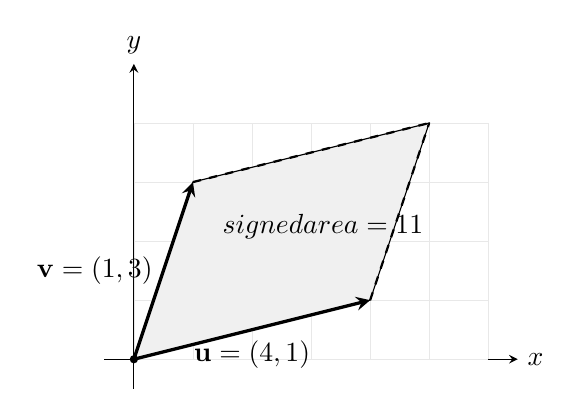
\begin{tikzpicture}[scale=0.75, >=stealth]
    \draw[->] (-0.5,0) -- (6.5,0) node[right] {\(x\)};
    \draw[->] (0,-0.5) -- (0,5.0) node[above] {\(y\)};
    \draw[step=1, gray!18, very thin] (0,0) grid (6,4);

    \coordinate (O) at (0,0);
    \coordinate (U) at (4,1);
    \coordinate (V) at (1,3);
    \coordinate (UV) at (5,4);

    \draw[fill=gray!12] (O) -- (U) -- (UV) -- (V) -- cycle;

    \draw[->, very thick] (O) -- (U) node[midway, below] {\(\mathbf u=(4,1)\)};
    \draw[->, very thick] (O) -- (V) node[midway, left] {\(\mathbf v=(1,3)\)};
    \draw[thick, dashed] (U) -- (UV);
    \draw[thick, dashed] (V) -- (UV);

    \node at (3.2,2.25) {\(\text{signed area}=11\)};

    \fill (O) circle (2pt);
\end{tikzpicture}
\caption{The determinant \(4\cdot3-1\cdot1=11\) is the signed area.}
\end{figure}

That expression
\[
    4\cdot3-1\cdot1
\]
is the determinant of the two vectors.

\begin{definition}[\(2\times2\) determinant]
If
\[
    \mathbf u=(u_1,u_2),
    \qquad
    \mathbf v=(v_1,v_2),
\]
then the \(2\times2\) determinant with columns \(\mathbf u\) and \(\mathbf v\) is
\[
\boxed{
    \det[\mathbf u\ \mathbf v]
    =
    \begin{vmatrix}
        u_1 & v_1\\
        u_2 & v_2
    \end{vmatrix}
    =
    u_1v_2-u_2v_1.
}
\]
\end{definition}

The vertical bars in
\[
    \begin{vmatrix}
        u_1 & v_1\\
        u_2 & v_2
    \end{vmatrix}
\]
do not mean absolute value.  They mean determinant.  A determinant can be positive,
negative, or zero.

\begin{theorem}[\(2\times2\) determinant as signed area]
For vectors
\[
    \mathbf u=(u_1,u_2),
    \qquad
    \mathbf v=(v_1,v_2),
\]
the determinant
\[
    \det[\mathbf u\ \mathbf v]
    =
    u_1v_2-u_2v_1
\]
is the signed area of the parallelogram spanned by \(\mathbf u\) and \(\mathbf v\).
\end{theorem}

\begin{proof}
Embed the plane in space by adding a zero \(z\)-coordinate:
\[
    \widetilde{\mathbf u}=(u_1,u_2,0),
    \qquad
    \widetilde{\mathbf v}=(v_1,v_2,0).
\]
Then
\[
    \widetilde{\mathbf u}\times\widetilde{\mathbf v}
    =
    (0,0,u_1v_2-u_2v_1).
\]
The cross product is the oriented area vector.  Its \(z\)-component is therefore the
signed area in the \(xy\)-plane:
\[
    u_1v_2-u_2v_1.
\]
\end{proof}

The sign contains orientation.

If
\[
    \mathbf u=(4,1),
    \qquad
    \mathbf v=(1,3),
\]
then
\[
    \det[\mathbf u\ \mathbf v]=11.
\]
But if we swap the order,
\[
    \det[\mathbf v\ \mathbf u]
    =
    \begin{vmatrix}
        1 & 4\\
        3 & 1
    \end{vmatrix}
    =
    1\cdot1-3\cdot4
    =
    -11.
\]
The parallelogram is the same.  The orientation is opposite.

If the two vectors are parallel, the determinant is zero.  For example,
\[
    \mathbf u=(1,2),
    \qquad
    \mathbf v=(2,4).
\]
Then
\[
    \det[\mathbf u\ \mathbf v]
    =
    \begin{vmatrix}
        1 & 2\\
        2 & 4
    \end{vmatrix}
    =
    1\cdot4-2\cdot2
    =
    0.
\]
The parallelogram has collapsed into a line segment.  Its area is zero.

\subsection{A square pushed into a parallelogram}

The determinant becomes especially useful when a whole grid is moved.

Suppose a machine sends the basic horizontal step
\[
    \mathbf e_1=(1,0)
\]
to
\[
    \mathbf u=(2,1),
\]
and sends the basic vertical step
\[
    \mathbf e_2=(0,1)
\]
to
\[
    \mathbf v=(1,3).
\]
The unit square becomes a parallelogram with signed area
\[
    \det[\mathbf u\ \mathbf v]
    =
    \begin{vmatrix}
        2 & 1\\
        1 & 3
    \end{vmatrix}
    =
    6-1
    =
    5.
\]
So this machine multiplies small signed areas by \(5\).

\begin{figure}[h]
\centering
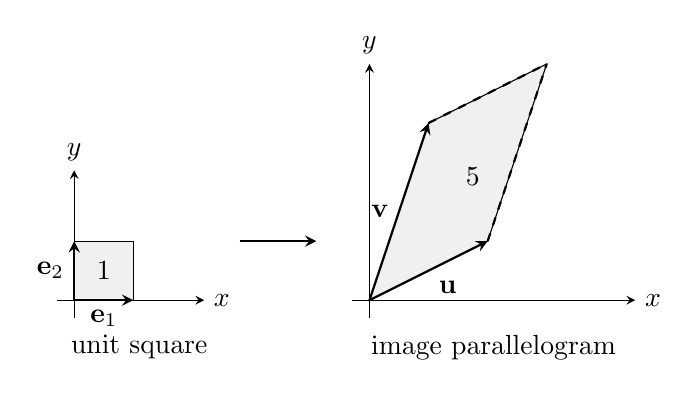
\begin{tikzpicture}[scale=0.75, >=stealth]
    \begin{scope}
        \draw[->] (-0.3,0) -- (2.2,0) node[right] {\(x\)};
        \draw[->] (0,-0.3) -- (0,2.2) node[above] {\(y\)};
        \draw[fill=gray!12] (0,0) -- (1,0) -- (1,1) -- (0,1) -- cycle;
        \draw[->, thick] (0,0) -- (1,0) node[midway, below] {\(\mathbf e_1\)};
        \draw[->, thick] (0,0) -- (0,1) node[midway, left] {\(\mathbf e_2\)};
        \node at (0.5,0.5) {\(1\)};
        \node at (1.1,-0.8) {unit square};
    \end{scope}

    \draw[->, thick] (2.8,1) -- (4.1,1);

    \begin{scope}[shift={(5,0)}]
        \draw[->] (-0.3,0) -- (4.5,0) node[right] {\(x\)};
        \draw[->] (0,-0.3) -- (0,4.0) node[above] {\(y\)};

        \coordinate (O) at (0,0);
        \coordinate (U) at (2,1);
        \coordinate (V) at (1,3);
        \coordinate (UV) at (3,4);

        \draw[fill=gray!12] (O) -- (U) -- (UV) -- (V) -- cycle;
        \draw[->, thick] (O) -- (U) node[midway, below right] {\(\mathbf u\)};
        \draw[->, thick] (O) -- (V) node[midway, left] {\(\mathbf v\)};
        \draw[thick, dashed] (U) -- (UV);
        \draw[thick, dashed] (V) -- (UV);
        \node at (1.75,2.1) {\(5\)};
        \node at (2.1,-0.8) {image parallelogram};
    \end{scope}
\end{tikzpicture}
\caption{A linear grid machine scales area by the determinant.}
\end{figure}

This idea will return in change of variables for double integrals.  When a coordinate
change bends and stretches a region, the determinant tells us the local area-scaling
factor.

\subsection{The \(3\times3\) determinant as signed volume}

In three dimensions, three vectors form a parallelepiped: a slanted box.

Take the simple case
\[
    \mathbf u=(2,0,0),
    \qquad
    \mathbf v=(0,3,0),
    \qquad
    \mathbf w=(0,0,4).
\]
They form a rectangular box with volume
\[
    2\cdot3\cdot4=24.
\]
The determinant gives the same number:
\[
    \begin{vmatrix}
        2 & 0 & 0\\
        0 & 3 & 0\\
        0 & 0 & 4
    \end{vmatrix}
    =
    24.
\]

Now tilt the box without changing its vertical height:
\[
    \mathbf u=(2,0,0),
    \qquad
    \mathbf v=(1,3,0),
    \qquad
    \mathbf w=(1,1,4).
\]
The volume is still \(24\).  The base parallelogram in the \(xy\)-plane has signed area
\[
    \begin{vmatrix}
        2 & 1\\
        0 & 3
    \end{vmatrix}
    =
    6,
\]
and the height is \(4\).  So the volume is
\[
    6\cdot4=24.
\]

The determinant packages this calculation into one number.

\begin{definition}[\(3\times3\) determinant]
If
\[
    \mathbf u=(u_1,u_2,u_3),
    \qquad
    \mathbf v=(v_1,v_2,v_3),
    \qquad
    \mathbf w=(w_1,w_2,w_3),
\]
then the \(3\times3\) determinant with columns \(\mathbf u,\mathbf v,\mathbf w\) is
\[
\boxed{
\det[\mathbf u\ \mathbf v\ \mathbf w]
=
\begin{vmatrix}
u_1 & v_1 & w_1\\
u_2 & v_2 & w_2\\
u_3 & v_3 & w_3
\end{vmatrix}
=
\mathbf u\cdot(\mathbf v\times\mathbf w).
}
\]
Expanded out,
\[
\begin{aligned}
\det[\mathbf u\ \mathbf v\ \mathbf w]
&=
u_1(v_2w_3-v_3w_2)\\
&\qquad
-v_1(u_2w_3-u_3w_2)\\
&\qquad
+w_1(u_2v_3-u_3v_2).
\end{aligned}
\]
\end{definition}

\begin{example}[A slanted box]
Let
\[
    \mathbf u=(2,0,0),
    \qquad
    \mathbf v=(1,3,0),
    \qquad
    \mathbf w=(1,1,4).
\]
Then
\[
\begin{aligned}
\det[\mathbf u\ \mathbf v\ \mathbf w]
&=
\mathbf u\cdot(\mathbf v\times\mathbf w).
\end{aligned}
\]
First compute
\[
\begin{aligned}
\mathbf v\times\mathbf w
&=
(1,3,0)\times(1,1,4)\\
&=
(3\cdot4-0\cdot1,\;0\cdot1-1\cdot4,\;1\cdot1-3\cdot1)\\
&=
(12,-4,-2).
\end{aligned}
\]
Then
\[
\begin{aligned}
\mathbf u\cdot(\mathbf v\times\mathbf w)
&=
(2,0,0)\cdot(12,-4,-2)\\
&=
24.
\end{aligned}
\]
So the signed volume is
\[
    24.
\]
\end{example}

\begin{figure}[h]
\centering
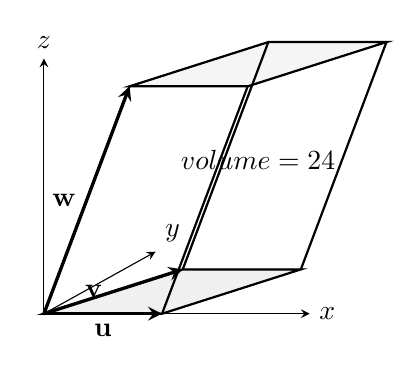
\begin{tikzpicture}[scale=0.75, >=stealth,
    x={(1cm,0cm)}, y={(0.45cm,0.25cm)}, z={(0cm,0.9cm)}]

    \coordinate (O) at (0,0,0);
    \coordinate (U) at (2,0,0);
    \coordinate (V) at (1,3,0);
    \coordinate (W) at (1,1,4);
    \coordinate (UV) at (3,3,0);
    \coordinate (UW) at (3,1,4);
    \coordinate (VW) at (2,4,4);
    \coordinate (UVW) at (4,4,4);

    \draw[->] (0,0,0) -- (4.5,0,0) node[right] {\(x\)};
    \draw[->] (0,0,0) -- (0,4.2,0) node[above right] {\(y\)};
    \draw[->] (0,0,0) -- (0,0,4.8) node[above] {\(z\)};

    \draw[fill=gray!12] (O) -- (U) -- (UV) -- (V) -- cycle;
    \draw[fill=gray!8] (W) -- (UW) -- (UVW) -- (VW) -- cycle;

    \draw[thick] (O) -- (U) -- (UV) -- (V) -- cycle;
    \draw[thick] (W) -- (UW) -- (UVW) -- (VW) -- cycle;
    \draw[thick] (O) -- (W);
    \draw[thick] (U) -- (UW);
    \draw[thick] (V) -- (VW);
    \draw[thick] (UV) -- (UVW);

    \draw[->, very thick] (O) -- (U) node[midway, below] {\(\mathbf u\)};
    \draw[->, very thick] (O) -- (V) node[midway, left] {\(\mathbf v\)};
    \draw[->, very thick] (O) -- (W) node[midway, left] {\(\mathbf w\)};

    \node at (2.5,2.5,2.2) {\(\text{volume}=24\)};
\end{tikzpicture}
\caption{Three vectors form a parallelepiped.  The determinant is its signed volume.}
\end{figure}

\subsection{Scalar triple product}

The expression
\[
    \mathbf u\cdot(\mathbf v\times\mathbf w)
\]
has a name.

\begin{definition}[Scalar triple product]
The \emph{scalar triple product} of three vectors in \(\mathbb R^3\) is
\[
\boxed{
    \mathbf u\cdot(\mathbf v\times\mathbf w).
}
\]
It is equal to the determinant
\[
    \det[\mathbf u\ \mathbf v\ \mathbf w].
\]
\end{definition}

The geometry is clean.  The vector
\[
    \mathbf v\times\mathbf w
\]
is an oriented area vector for the base parallelogram spanned by \(\mathbf v\) and
\(\mathbf w\).  Dotting with \(\mathbf u\) takes the component of \(\mathbf u\) in the
normal direction and multiplies by that base area.  That is base area times signed
height.

\begin{theorem}[Scalar triple product as signed volume]
The signed volume of the parallelepiped spanned by
\[
    \mathbf u,\mathbf v,\mathbf w
\]
is
\[
\boxed{
    \mathbf u\cdot(\mathbf v\times\mathbf w).
}
\]
The ordinary volume is
\[
\boxed{
    \left|\mathbf u\cdot(\mathbf v\times\mathbf w)\right|.
}
\]
\end{theorem}

\begin{proof}
The vector \(\mathbf v\times\mathbf w\) is perpendicular to the base parallelogram
spanned by \(\mathbf v\) and \(\mathbf w\), and its length is the area of that base.

If \(\mathbf v\times\mathbf w\neq\mathbf 0\), then
\[
    \widehat{\mathbf n}
    =
    \frac{\mathbf v\times\mathbf w}{\|\mathbf v\times\mathbf w\|}
\]
is a unit normal to the base.  The signed height of \(\mathbf u\) above the base is
\[
    \mathbf u\cdot\widehat{\mathbf n}.
\]
So the signed volume is
\[
\begin{aligned}
\text{base area}\cdot\text{signed height}
&=
\|\mathbf v\times\mathbf w\|
\left(
\mathbf u\cdot
\frac{\mathbf v\times\mathbf w}{\|\mathbf v\times\mathbf w\|}
\right)\\
&=
\mathbf u\cdot(\mathbf v\times\mathbf w).
\end{aligned}
\]

If \(\mathbf v\times\mathbf w=\mathbf 0\), then \(\mathbf v\) and \(\mathbf w\) are
parallel, so the base has zero area.  The parallelepiped has volume \(0\), and the
formula also gives
\[
    \mathbf u\cdot(\mathbf v\times\mathbf w)
    =
    \mathbf u\cdot\mathbf 0
    =
    0.
\]
\end{proof}

The proof divided by
\[
    \|\mathbf v\times\mathbf w\|
\]
only when this number was not zero.  That condition matters.  If
\[
    \mathbf v=(1,0,0),
    \qquad
    \mathbf w=(2,0,0),
\]
then
\[
    \mathbf v\times\mathbf w=\mathbf 0,
\]
so the unit normal
\[
    \frac{\mathbf v\times\mathbf w}{\|\mathbf v\times\mathbf w\|}
\]
is meaningless.  But the volume formula survives:
\[
    \mathbf u\cdot(\mathbf v\times\mathbf w)=0.
\]
The box has collapsed because two of its edges point along the same line.

\subsection{Orientation of ordered bases}

The sign of a determinant tells us orientation.

The standard ordered basis in space is
\[
    \mathbf i=(1,0,0),
    \qquad
    \mathbf j=(0,1,0),
    \qquad
    \mathbf k=(0,0,1).
\]
Its determinant is
\[
    \det[\mathbf i\ \mathbf j\ \mathbf k]
    =
    \begin{vmatrix}
    1&0&0\\
    0&1&0\\
    0&0&1
    \end{vmatrix}
    =
    1.
\]
So
\[
    (\mathbf i,\mathbf j,\mathbf k)
\]
is positively oriented.

If we swap the first two vectors, we get
\[
    (\mathbf j,\mathbf i,\mathbf k).
\]
Its determinant is
\[
    \det[\mathbf j\ \mathbf i\ \mathbf k]
    =
    \begin{vmatrix}
    0&1&0\\
    1&0&0\\
    0&0&1
    \end{vmatrix}
    =
    -1.
\]
The volume is still \(1\), but the orientation has reversed.

\begin{definition}[Orientation of an ordered basis in \(\mathbb R^3\)]
An ordered triple of vectors
\[
    (\mathbf u,\mathbf v,\mathbf w)
\]
is a \emph{basis} of \(\mathbb R^3\) if the vectors are independent, so that their
parallelepiped has nonzero volume.

The basis is \emph{positively oriented} if
\[
    \det[\mathbf u\ \mathbf v\ \mathbf w]>0.
\]
It is \emph{negatively oriented} if
\[
    \det[\mathbf u\ \mathbf v\ \mathbf w]<0.
\]
\end{definition}

The word \emph{basis} matters.  If
\[
    \mathbf u=(1,0,0),
    \qquad
    \mathbf v=(0,1,0),
    \qquad
    \mathbf w=(1,0,0),
\]
then the determinant is
\[
    \det[\mathbf u\ \mathbf v\ \mathbf w]=0.
\]
These three vectors do not fill space.  They lie in the same plane because
\[
    \mathbf w=\mathbf u.
\]
So the triple has no positive or negative orientation as a basis.  It is not a basis at all.

The same idea works in the plane.  The ordered pair
\[
    ((1,0),(0,1))
\]
is positively oriented because
\[
    \begin{vmatrix}
    1&0\\
    0&1
    \end{vmatrix}
    =
    1.
\]
The ordered pair
\[
    ((0,1),(1,0))
\]
is negatively oriented because
\[
    \begin{vmatrix}
    0&1\\
    1&0
    \end{vmatrix}
    =
    -1.
\]

Orientation is the mathematical version of choosing clockwise versus
counterclockwise in the plane, or right-handed versus left-handed in space.

\subsection{Determinants as volume-scaling factors}

A determinant does not only measure one parallelogram or one parallelepiped.  It
measures how a linear machine scales area or volume.

Consider the plane machine
\[
    T(x,y)=x(2,1)+y(1,3).
\]
It sends
\[
    (1,0)\mapsto (2,1),
    \qquad
    (0,1)\mapsto (1,3).
\]
So it sends the unit square to the parallelogram spanned by
\[
    \mathbf u=(2,1),
    \qquad
    \mathbf v=(1,3).
\]
The determinant is
\[
    \det[\mathbf u\ \mathbf v]
    =
    \begin{vmatrix}
        2&1\\
        1&3
    \end{vmatrix}
    =
    5.
\]
Therefore the machine multiplies signed area by \(5\).

A tiny rectangle with side lengths
\[
    \Delta x
    \qquad\text{and}\qquad
    \Delta y
\]
has area
\[
    \Delta x\,\Delta y.
\]
After applying \(T\), it becomes a tiny parallelogram with area
\[
    5\,\Delta x\,\Delta y.
\]

In space, if a machine sends the coordinate steps
\[
    \mathbf i,\mathbf j,\mathbf k
\]
to
\[
    \mathbf u,\mathbf v,\mathbf w,
\]
then it sends the unit cube to the parallelepiped spanned by
\[
    \mathbf u,\mathbf v,\mathbf w.
\]
The signed volume scaling factor is
\[
    \det[\mathbf u\ \mathbf v\ \mathbf w].
\]

\begin{example}[A shear preserves area]
Let
\[
    T(x,y)=(x+2y,y).
\]
Then
\[
    T(1,0)=(1,0),
    \qquad
    T(0,1)=(2,1).
\]
The area scaling factor is
\[
    \begin{vmatrix}
        1&2\\
        0&1
    \end{vmatrix}
    =
    1.
\]
This machine slants squares into parallelograms, but it preserves area.

A square can be pushed sideways without changing its area.  The determinant sees
that.
\end{example}

\begin{example}[A coordinate stretch changes volume]
Let a space machine stretch \(x\)-distances by \(2\), \(y\)-distances by \(3\), and
\(z\)-distances by \(4\):
\[
    T(x,y,z)=(2x,3y,4z).
\]
Then
\[
    T(\mathbf i)=(2,0,0),
    \qquad
    T(\mathbf j)=(0,3,0),
    \qquad
    T(\mathbf k)=(0,0,4).
\]
The volume scaling factor is
\[
    \begin{vmatrix}
    2&0&0\\
    0&3&0\\
    0&0&4
    \end{vmatrix}
    =
    24.
\]
So every small volume is multiplied by \(24\).
\end{example}

This is why determinants appear in change of variables.  When we later replace
\((x,y)\) by better coordinates, the determinant will tell us how much each little area
piece has been stretched.  In polar coordinates, that mysterious extra factor
\[
    r
\]
in
\[
    dA=r\,dr\,d\theta
\]
will turn out to be a determinant.

But the determinant has revealed something even more basic: area and volume change
sign when we swap directions.  Ordinary multiplication does not behave that way:
\[
    ab=ba.
\]
Oriented area does:
\[
    \det[\mathbf u\ \mathbf v]=-\det[\mathbf v\ \mathbf u].
\]
That sign flip is not a technicality.  It is the beginning of a new product, built for
oriented geometry.  The next section gives it a name: the wedge product.
\section{Alternating products: a first glimpse of forms}

The determinant gave us signed area and signed volume.  That sign was not decoration.
It was the whole point.  When we swapped two directions, the parallelogram stayed the
same, but its orientation reversed:
\[
    \det[\mathbf u\ \mathbf v]
    =
    -\det[\mathbf v\ \mathbf u].
\]
Now we give that sign-changing behavior a name.  It is the first step toward
differential forms.

\subsection{Area as a bilinear alternating measurement}

A carpenter lays a small slanted tile on the floor.  One side of the tile follows the vector
\[
    \mathbf u=(3,1),
\]
and the adjacent side follows
\[
    \mathbf v=(1,2).
\]
The signed area of the parallelogram is
\[
    \det[\mathbf u\ \mathbf v]
    =
    \begin{vmatrix}
        3&1\\
        1&2
    \end{vmatrix}
    =
    3\cdot2-1\cdot1
    =
    5.
\]

The tile has ordinary area \(5\).  It also has positive orientation because the ordered
pair
\[
    \mathbf u,\mathbf v
\]
turns counterclockwise.

If we walk around the same tile in the opposite order, the signed area becomes
\[
    \det[\mathbf v\ \mathbf u]
    =
    \begin{vmatrix}
        1&3\\
        2&1
    \end{vmatrix}
    =
    1\cdot1-2\cdot3
    =
    -5.
\]
The tile did not shrink.  Only the orientation changed.

\begin{figure}[h]
\centering
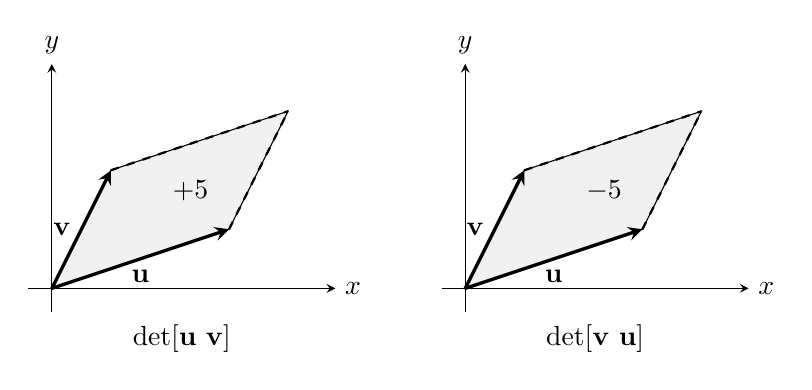
\begin{tikzpicture}[scale=0.75, >=stealth]
    \begin{scope}
        \draw[->] (-0.4,0) -- (4.8,0) node[right] {\(x\)};
        \draw[->] (0,-0.4) -- (0,3.8) node[above] {\(y\)};
        \coordinate (O) at (0,0);
        \coordinate (U) at (3,1);
        \coordinate (V) at (1,2);
        \coordinate (UV) at (4,3);

        \draw[fill=gray!12] (O) -- (U) -- (UV) -- (V) -- cycle;
        \draw[->, very thick] (O) -- (U) node[midway, below] {\(\mathbf u\)};
        \draw[->, very thick] (O) -- (V) node[midway, left] {\(\mathbf v\)};
        \draw[thick, dashed] (U) -- (UV);
        \draw[thick, dashed] (V) -- (UV);
        \node at (2.35,1.65) {\(+5\)};
        \node at (2.2,-0.85) {\(\det[\mathbf u\ \mathbf v]\)};
    \end{scope}

    \begin{scope}[shift={(7,0)}]
        \draw[->] (-0.4,0) -- (4.8,0) node[right] {\(x\)};
        \draw[->] (0,-0.4) -- (0,3.8) node[above] {\(y\)};
        \coordinate (O) at (0,0);
        \coordinate (U) at (3,1);
        \coordinate (V) at (1,2);
        \coordinate (UV) at (4,3);

        \draw[fill=gray!12] (O) -- (V) -- (UV) -- (U) -- cycle;
        \draw[->, very thick] (O) -- (V) node[midway, left] {\(\mathbf v\)};
        \draw[->, very thick] (O) -- (U) node[midway, below] {\(\mathbf u\)};
        \draw[thick, dashed] (U) -- (UV);
        \draw[thick, dashed] (V) -- (UV);
        \node at (2.35,1.65) {\(-5\)};
        \node at (2.2,-0.85) {\(\det[\mathbf v\ \mathbf u]\)};
    \end{scope}
\end{tikzpicture}
\caption{The same parallelogram has opposite signed area when the order is reversed.}
\end{figure}

The determinant also behaves linearly in each input.  For example, split
\[
    \mathbf u=(3,1)
\]
into
\[
    \mathbf u=(3,0)+(0,1).
\]
Then
\[
\begin{aligned}
\det[(3,1)\ \mathbf v]
&=
\det[(3,0)\ \mathbf v]
+
\det[(0,1)\ \mathbf v].
\end{aligned}
\]
With \(\mathbf v=(1,2)\), this says
\[
    5
    =
    \begin{vmatrix}
        3&1\\
        0&2
    \end{vmatrix}
    +
    \begin{vmatrix}
        0&1\\
        1&2
    \end{vmatrix}
    =
    6+(-1).
\]
So signed area is additive in the first vector.  It is also additive in the second vector.
Stretch one side by a factor of \(c\), and the signed area is stretched by the same factor.

This is the pattern.

\begin{definition}[Bilinear and alternating]
A function \(B(\mathbf u,\mathbf v)\) that takes two vectors and returns a number is
called \emph{bilinear} if it is linear in each input separately:
\[
    B(a\mathbf u+b\mathbf w,\mathbf v)
    =
    aB(\mathbf u,\mathbf v)+bB(\mathbf w,\mathbf v),
\]
and
\[
    B(\mathbf u,a\mathbf v+b\mathbf w)
    =
    aB(\mathbf u,\mathbf v)+bB(\mathbf u,\mathbf w).
\]

It is called \emph{alternating} if swapping the two inputs changes the sign:
\[
    B(\mathbf v,\mathbf u)=-B(\mathbf u,\mathbf v).
\]
In particular,
\[
    B(\mathbf u,\mathbf u)=0.
\]
\end{definition}

The determinant in the plane is bilinear and alternating:
\[
    \det[\mathbf u\ \mathbf v]=u_1v_2-u_2v_1.
\]

\begin{theorem}[Every planar alternating bilinear measurement is area times a constant]
Let \(B\) be a bilinear alternating function of two vectors in \(\mathbb R^2\).  Then
there is a constant \(c\) such that
\[
\boxed{
    B(\mathbf u,\mathbf v)
    =
    c(u_1v_2-u_2v_1)
}
\]
for all
\[
    \mathbf u=(u_1,u_2),
    \qquad
    \mathbf v=(v_1,v_2).
\]
In other words, every bilinear alternating measurement in the plane is a constant
multiple of signed area.
\end{theorem}

\begin{proof}
Let
\[
    \mathbf e_1=(1,0),
    \qquad
    \mathbf e_2=(0,1).
\]
Write
\[
    \mathbf u=u_1\mathbf e_1+u_2\mathbf e_2,
    \qquad
    \mathbf v=v_1\mathbf e_1+v_2\mathbf e_2.
\]
By bilinearity,
\[
\begin{aligned}
B(\mathbf u,\mathbf v)
&=
B(u_1\mathbf e_1+u_2\mathbf e_2,\,
  v_1\mathbf e_1+v_2\mathbf e_2)\\
&=
u_1v_1B(\mathbf e_1,\mathbf e_1)
+u_1v_2B(\mathbf e_1,\mathbf e_2)\\
&\qquad
+u_2v_1B(\mathbf e_2,\mathbf e_1)
+u_2v_2B(\mathbf e_2,\mathbf e_2).
\end{aligned}
\]
Because \(B\) is alternating,
\[
    B(\mathbf e_1,\mathbf e_1)=0,
    \qquad
    B(\mathbf e_2,\mathbf e_2)=0,
\]
and
\[
    B(\mathbf e_2,\mathbf e_1)
    =
    -B(\mathbf e_1,\mathbf e_2).
\]
Let
\[
    c=B(\mathbf e_1,\mathbf e_2).
\]
Then
\[
\begin{aligned}
B(\mathbf u,\mathbf v)
&=
u_1v_2c-u_2v_1c\\
&=
c(u_1v_2-u_2v_1).
\end{aligned}
\]
\end{proof}

The two hypotheses are real hypotheses.

First, bilinearity matters.  Define
\[
    B(\mathbf u,\mathbf v)
    =
    (u_1v_2-u_2v_1)^3.
\]
Swapping \(\mathbf u\) and \(\mathbf v\) changes the sign, so this function is
alternating.  But it is not bilinear.  For example,
\[
    B(\mathbf e_1,\mathbf e_2)=1,
\]
while
\[
    B(2\mathbf e_1,\mathbf e_2)=8.
\]
A bilinear function would have given \(2\), not \(8\).  So this is not a constant
multiple of signed area.

Second, alternating matters.  The dot product
\[
    D(\mathbf u,\mathbf v)=\mathbf u\cdot\mathbf v
\]
is bilinear, but it is not alternating.  Indeed,
\[
    D(\mathbf e_1,\mathbf e_1)=1,
\]
while an alternating measurement must give
\[
    B(\mathbf e_1,\mathbf e_1)=0.
\]
The dot product measures alignment, not oriented area.

\subsection{The coordinate measurements \(dx\), \(dy\), and \(dz\)}

The determinant formula
\[
    u_1v_2-u_2v_1
\]
has two parts.  It uses the \(x\)-component of one vector and the \(y\)-component of
the other, then subtracts the same measurement with the roles reversed.

To name those component measurements, we write
\[
    dx(a,b)=a,
    \qquad
    dy(a,b)=b.
\]
So \(dx\) reads the \(x\)-component of a vector, and \(dy\) reads the \(y\)-component.

For example, if
\[
    \mathbf u=(3,1),
    \qquad
    \mathbf v=(1,2),
\]
then
\[
    dx(\mathbf u)=3,
    \qquad
    dy(\mathbf u)=1,
\]
and
\[
    dx(\mathbf v)=1,
    \qquad
    dy(\mathbf v)=2.
\]

These are the first examples of \emph{1-forms}: objects that take one vector and return
one number.  Later, a 1-form like
\[
    P\,dx+Q\,dy
\]
will be the kind of object we integrate along a curve.  For now, \(dx\) and \(dy\)
are simply coordinate-measuring devices.

In space we also have
\[
    dz(a,b,c)=c.
\]

\subsection{Why \(dx\,dy\) should not mean ordinary multiplication}

A parallelogram has two side vectors.  So an area measurement must take two vector
inputs, not one.

If
\[
    \mathbf u=(3,1),
    \qquad
    \mathbf v=(1,2),
\]
then ordinary multiplication might tempt us to write
\[
    dx(\mathbf u)\,dy(\mathbf v)=3\cdot2=6.
\]
But the signed area is not \(6\).  It is
\[
    3\cdot2-1\cdot1=5.
\]
The missing piece is the swapped product:
\[
    dy(\mathbf u)\,dx(\mathbf v)=1\cdot1=1.
\]
Signed area is the difference:
\[
    dx(\mathbf u)\,dy(\mathbf v)-dy(\mathbf u)\,dx(\mathbf v).
\]

This difference is important enough to get its own symbol.

\begin{definition}[The wedge product \(dx\wedge dy\)]
The wedge product \(dx\wedge dy\) is the signed area measurement defined by
\[
\boxed{
    (dx\wedge dy)(\mathbf u,\mathbf v)
    =
    dx(\mathbf u)dy(\mathbf v)
    -
    dy(\mathbf u)dx(\mathbf v).
}
\]
If
\[
    \mathbf u=(u_1,u_2),
    \qquad
    \mathbf v=(v_1,v_2),
\]
then
\[
\boxed{
    (dx\wedge dy)(\mathbf u,\mathbf v)
    =
    u_1v_2-u_2v_1.
}
\]
\end{definition}

So
\[
    dx\wedge dy
\]
is not ordinary multiplication.  The wedge symbol \(\wedge\) is a warning:
\[
    \text{measure the ordered area, and subtract the swapped order.}
\]

The sign rule is immediate:
\[
\boxed{
    dx\wedge dy=-dy\wedge dx.
}
\]
Also,
\[
\boxed{
    dx\wedge dx=0,
    \qquad
    dy\wedge dy=0.
}
\]
A vector and itself span no area.

This is why the notation \(dx\,dy\) is too quiet when orientation matters.  In ordinary
double integrals, \(dA\) often means unsigned little area.  But the form
\[
    dx\wedge dy
\]
remembers orientation.  Reversing the order reverses the sign.

\subsection{Coordinate shadows in space}

A parallelogram in space casts shadows onto the coordinate planes.  Each shadow has
a signed area.

Let
\[
    \mathbf u=(2,1,3),
    \qquad
    \mathbf v=(1,4,0).
\]
The signed area of the shadow on the \(xy\)-plane is
\[
\begin{aligned}
(dx\wedge dy)(\mathbf u,\mathbf v)
&=
\begin{vmatrix}
2&1\\
1&4
\end{vmatrix}\\
&=
2\cdot4-1\cdot1\\
&=
7.
\end{aligned}
\]

The signed area of the shadow on the \(yz\)-plane is
\[
\begin{aligned}
(dy\wedge dz)(\mathbf u,\mathbf v)
&=
\begin{vmatrix}
1&4\\
3&0
\end{vmatrix}\\
&=
1\cdot0-3\cdot4\\
&=
-12.
\end{aligned}
\]

The signed area of the shadow on the \(zx\)-plane is
\[
\begin{aligned}
(dz\wedge dx)(\mathbf u,\mathbf v)
&=
\begin{vmatrix}
3&0\\
2&1
\end{vmatrix}\\
&=
3\cdot1-2\cdot0\\
&=
3.
\end{aligned}
\]

Now compute the cross product:
\[
\begin{aligned}
\mathbf u\times\mathbf v
&=
(2,1,3)\times(1,4,0)\\
&=
(1\cdot0-3\cdot4,\;3\cdot1-2\cdot0,\;2\cdot4-1\cdot1)\\
&=
(-12,3,7).
\end{aligned}
\]
So the cross product has been secretly collecting the three signed shadow areas:
\[
\boxed{
\mathbf u\times\mathbf v
=
\bigl(
(dy\wedge dz)(\mathbf u,\mathbf v),\,
(dz\wedge dx)(\mathbf u,\mathbf v),\,
(dx\wedge dy)(\mathbf u,\mathbf v)
\bigr).
}
\]

This is a beautiful fact.  The cross product packages three coordinate area measurements
into one vector.  But the area measurements themselves are the wedge products.

That is why the wedge product survives in every dimension, while the cross product is
special to three dimensions.

\subsection{Signed volume as \(dx\wedge dy\wedge dz\)}

The same idea works for volume.

A signed volume measurement takes three vectors.  It is linear in each input and changes
sign whenever two inputs are swapped.

The basic signed volume measurement in space is
\[
    dx\wedge dy\wedge dz.
\]

\begin{definition}[The volume form \(dx\wedge dy\wedge dz\)]
For vectors
\[
    \mathbf u,\mathbf v,\mathbf w\in\mathbb R^3,
\]
the form \(dx\wedge dy\wedge dz\) is defined by
\[
\boxed{
    (dx\wedge dy\wedge dz)(\mathbf u,\mathbf v,\mathbf w)
    =
    \det[\mathbf u\ \mathbf v\ \mathbf w].
}
\]
It measures the signed volume of the parallelepiped spanned by the ordered triple
\[
    \mathbf u,\mathbf v,\mathbf w.
\]
\end{definition}

For example, let
\[
    \mathbf u=(1,2,0),
    \qquad
    \mathbf v=(0,1,3),
    \qquad
    \mathbf w=(2,0,1).
\]
Then
\[
\begin{aligned}
(dx\wedge dy\wedge dz)(\mathbf u,\mathbf v,\mathbf w)
&=
\begin{vmatrix}
1&0&2\\
2&1&0\\
0&3&1
\end{vmatrix}\\
&=
13.
\end{aligned}
\]
So the ordered triple spans signed volume \(13\).

If we swap the first two vectors, the sign flips:
\[
    (dx\wedge dy\wedge dz)(\mathbf v,\mathbf u,\mathbf w)
    =
    -13.
\]
Again, the box is the same.  The orientation is not.

\subsection{Forms as future integrands}

The word \emph{form} may sound abstract, but at this stage it means something very
concrete.

A 1-form measures a vector:
\[
    dx,
    \qquad
    dy,
    \qquad
    P\,dx+Q\,dy.
\]
Later, 1-forms will be integrated along curves.

A 2-form measures oriented area:
\[
    dx\wedge dy,
    \qquad
    dy\wedge dz,
    \qquad
    dz\wedge dx.
\]
Later, 2-forms will be integrated over surfaces and regions.

A 3-form measures oriented volume:
\[
    dx\wedge dy\wedge dz.
\]
Later, 3-forms will be integrated over solids.

So the wedge product is not a new trick for multiplying symbols.  It is a way to keep
track of oriented geometry:
\[
    \text{length, area, volume, and the signs that come from order.}
\]

This chapter began with Hamilton trying to multiply directions.  It ends with a different
kind of product, one that does not try to turn area into a vector.  It lets area be area.
Before these forms become integrals, one more piece of machinery has to arrive.  We
need rules that move every vector in a grid at once.  Those rules are linear maps, and
their bookkeeping devices are matrices.

\section{Chapter review and discovery problems}

Hamilton's multiplication led us to the dot product and cross product.  Determinants
then pulled out the deeper quantities: signed area and signed volume.  The wedge
product kept those quantities in their natural form.

This review is not meant to be a list of formulas to memorize.  The goal is to keep the
geometric story alive while practicing the computations.

\subsection{Concept check}

\begin{enumerate}
\item Explain the difference between a point and a vector.  Why can the same ordered
pair represent either one, depending on context?

\item Complex multiplication by
\[
    re^{i\theta}
\]
has two geometric effects.  What are they?

\item Why did Hamilton have to give up commutativity when he introduced the quaternion
units \(i,j,k\)?

\item The quaternion rules include
\[
    ij=k,
    \qquad
    ji=-k.
\]
What geometric idea is hidden in this sign change?

\item When two pure imaginary quaternions
\[
    U=u_1i+u_2j+u_3k,
    \qquad
    V=v_1i+v_2j+v_3k
\]
are multiplied, their product splits as
\[
    UV=-\mathbf u\cdot\mathbf v+\mathbf u\times\mathbf v.
\]
Which part measures alignment?  Which part measures oriented area?

\item What does
\[
    \mathbf u\cdot\mathbf v=0
\]
mean geometrically, assuming neither vector is zero?

\item What does
\[
    \mathbf u\times\mathbf v=\mathbf 0
\]
mean geometrically?

\item Why does the cross product point perpendicular to the parallelogram spanned by
its inputs?

\item Explain why
\[
    \det[\mathbf u\ \mathbf v]
\]
is signed area, not just area.

\item Explain why
\[
    \det[\mathbf u\ \mathbf v\ \mathbf w]=0
\]
means that the three vectors do not form a genuine three-dimensional box.

\item What does it mean for an ordered basis of \(\mathbb R^3\) to be positively
oriented?

\item Why is there no single honest cross product for two vectors in \(\mathbb R^4\)?
What goes wrong with the idea of ``the perpendicular direction''?

\item What is the geometric meaning of
\[
    dx\wedge dy=-dy\wedge dx?
\]

\item Why is
\[
    dx\wedge dx=0?
\]
\end{enumerate}

\subsection{Skills}

\begin{enumerate}
\item Compute and interpret geometrically:
\[
    (2+3i)(1-i).
\]
Write the answer in rectangular form.

\item Write
\[
    -1+i\sqrt3
\]
in polar form.  What rotation and scaling does multiplication by this complex number
perform?

\item Use the quaternion rules to compute
\[
    (2i-j+3k)(i+4j+2k).
\]
Then identify the scalar part and the vector part.

\item Let
\[
    \mathbf u=(3,4,0),
    \qquad
    \mathbf v=(1,2,2).
\]
Compute
\[
    \mathbf u\cdot\mathbf v,
    \qquad
    \|\mathbf u\|,
    \qquad
    \|\mathbf v\|,
\]
and the cosine of the angle between them.

\item Find the projection of
\[
    \mathbf u=(3,4,0)
\]
onto
\[
    \mathbf v=(1,2,2).
\]

\item A sled is pulled by a force
\[
    \mathbf F=(30,10)
\]
newtons through a displacement
\[
    \mathbf d=(8,6)
\]
meters.  Compute the work done:
\[
    W=\mathbf F\cdot\mathbf d.
\]

\item Compute
\[
    (2,-1,3)\times(1,4,2).
\]
Then check directly that your answer is perpendicular to both input vectors.

\item Find a normal vector to the plane spanned by
\[
    \mathbf a=(1,2,0),
    \qquad
    \mathbf b=(0,1,3).
\]

\item Find an equation of the plane through
\[
    P=(2,-1,4)
\]
with direction vectors
\[
    \mathbf a=(1,2,0),
    \qquad
    \mathbf b=(0,1,3).
\]

\item A force
\[
    \mathbf F=(0,40,0)
\]
is applied at position
\[
    \mathbf r=(0.25,0,0)
\]
meters from a pivot.  Compute the torque
\[
    \boldsymbol\tau=\mathbf r\times\mathbf F.
\]

\item Compute the signed area:
\[
    \begin{vmatrix}
        5&2\\
        1&4
    \end{vmatrix}.
\]
Then interpret the sign.

\item Find the area of the triangle with vertices
\[
    A=(1,1),
    \qquad
    B=(5,2),
    \qquad
    C=(2,6).
\]
Hint: first find the parallelogram area spanned by
\[
    B-A
    \qquad\text{and}\qquad
    C-A.
\]

\item Compute the signed volume:
\[
    \begin{vmatrix}
        1&0&2\\
        2&1&0\\
        0&3&1
    \end{vmatrix}.
\]

\item Find the volume of the tetrahedron with vertices
\[
    A=(0,0,0),
    \qquad
    B=(1,2,0),
    \qquad
    C=(0,1,3),
    \qquad
    D=(2,0,1).
\]
Hint: a tetrahedron has one-sixth the volume of the parallelepiped formed by its three
edge vectors from one vertex.

\item A linear grid machine sends
\[
    \mathbf e_1=(1,0)
    \quad\text{to}\quad
    \mathbf u=(3,1),
\]
and
\[
    \mathbf e_2=(0,1)
    \quad\text{to}\quad
    \mathbf v=(2,4).
\]
Find the signed area-scaling factor of the machine.

\item Decide whether the machine in the previous problem preserves orientation, reverses
orientation, or collapses area.

\item Compute
\[
    (dx\wedge dy)(\mathbf u,\mathbf v)
\]
for
\[
    \mathbf u=(4,-1),
    \qquad
    \mathbf v=(2,3).
\]

\item For
\[
    \mathbf u=(2,1,3),
    \qquad
    \mathbf v=(1,4,0),
\]
compute the three signed shadow areas
\[
    (dy\wedge dz)(\mathbf u,\mathbf v),
\]
\[
    (dz\wedge dx)(\mathbf u,\mathbf v),
\]
and
\[
    (dx\wedge dy)(\mathbf u,\mathbf v).
\]
Then compare them with the components of \(\mathbf u\times\mathbf v\).

\item Decide whether each ordered triple is positively oriented, negatively oriented, or
not a basis:
\[
    (\mathbf i,\mathbf j,\mathbf k),
\]
\[
    (\mathbf j,\mathbf i,\mathbf k),
\]
\[
    (\mathbf i,\mathbf j,\mathbf i+\mathbf j),
\]
\[
    (\mathbf i+\mathbf j,\mathbf j+\mathbf k,\mathbf k+\mathbf i).
\]
\end{enumerate}

\subsection{Discovery problems}

\begin{enumerate}
\item Let
\[
    \mathbf u=(u_1,u_2,u_3),
    \qquad
    \mathbf v=(v_1,v_2,v_3).
\]
Show that the components of \(\mathbf u\times\mathbf v\) are the three signed shadow
areas:
\[
\mathbf u\times\mathbf v
=
\bigl(
(dy\wedge dz)(\mathbf u,\mathbf v),\,
(dz\wedge dx)(\mathbf u,\mathbf v),\,
(dx\wedge dy)(\mathbf u,\mathbf v)
\bigr).
\]

\item Use the previous problem to show that
\[
\|\mathbf u\times\mathbf v\|^2
=
\bigl((dy\wedge dz)(\mathbf u,\mathbf v)\bigr)^2
+
\bigl((dz\wedge dx)(\mathbf u,\mathbf v)\bigr)^2
+
\bigl((dx\wedge dy)(\mathbf u,\mathbf v)\bigr)^2.
\]
This says that the squared area of a parallelogram in space is the sum of the squared
areas of its coordinate shadows.

\item Show directly from the quaternion product that
\[
    UV+VU=-2\,\mathbf u\cdot\mathbf v.
\]
This identity says that the dot product is the symmetric part of the product.

\item Show directly from the quaternion product that
\[
    UV-VU=2\,\mathbf u\times\mathbf v.
\]
This identity says that the cross product is the antisymmetric part of the product.

\item Let
\[
    B(\mathbf u,\mathbf v)=u_1v_2-u_2v_1.
\]
Prove directly from the formula that \(B\) is bilinear and alternating.

\item Let
\[
    C(\mathbf u,\mathbf v)=u_1v_1+u_2v_2.
\]
Prove directly from the formula that \(C\) is bilinear but not alternating.

\item Let
\[
    A(\mathbf u,\mathbf v)=(u_1v_2-u_2v_1)^3.
\]
Show that \(A\) is alternating but not bilinear.

\item In \(\mathbb R^4\), let
\[
    \mathbf e_1=(1,0,0,0),
    \qquad
    \mathbf e_2=(0,1,0,0).
\]
Find two different unit vectors perpendicular to both \(\mathbf e_1\) and
\(\mathbf e_2\).  Explain why this prevents a unique normal-vector cross product for
two vectors in \(\mathbb R^4\).

\item The determinant changes sign when two columns are swapped.  Use this fact to
explain why
\[
    dx\wedge dy\wedge dz
\]
changes sign whenever two input vectors are swapped.

\item A small polar coordinate rectangle has sides
\[
    \Delta r
    \qquad\text{and}\qquad
    r\,\Delta\theta
\]
when it is located at radius \(r\).  Use this to explain why the polar area element will
later contain the factor
\[
    r:
\]
\[
    dA=r\,dr\,d\theta.
\]
Where does the \(r\) come from geometrically?

\item A machine sends the unit square to the parallelogram spanned by
\[
    \mathbf u=(a,c),
    \qquad
    \mathbf v=(b,d).
\]
Show that its signed area-scaling factor is
\[
    ad-bc.
\]
This number will become the determinant of the matrix
\[
    \begin{pmatrix}
    a&b\\
    c&d
    \end{pmatrix}.
\]

\item Suppose a machine in space sends
\[
    \mathbf i,\mathbf j,\mathbf k
\]
to
\[
    \mathbf u,\mathbf v,\mathbf w.
\]
Explain why the signed volume-scaling factor must be
\[
    \det[\mathbf u\ \mathbf v\ \mathbf w].
\]

\item Let
\[
    \mathbf u=(1,2,0),
    \qquad
    \mathbf v=(0,1,3),
    \qquad
    \mathbf w=(2,0,1).
\]
Compute
\[
    (dx\wedge dy\wedge dz)(\mathbf u,\mathbf v,\mathbf w).
\]
Then swap two of the vectors and compute again.  What changes?  What stays the same?

\item Find two different ordered bases of \(\mathbb R^3\) that span boxes with the same
ordinary volume but opposite orientation.

\item A parallelogram in space has side vectors \(\mathbf u\) and \(\mathbf v\).  Its
cross product \(\mathbf u\times\mathbf v\) packages the coordinate shadow areas into
a vector.  But in \(\mathbb R^4\), there are six coordinate-plane shadows:
\[
    dx\wedge dy,\quad dx\wedge dz,\quad dx\wedge dw,\quad
    dy\wedge dz,\quad dy\wedge dw,\quad dz\wedge dw.
\]
What does this suggest about why a single normal vector is not enough to represent
oriented area in four dimensions?
\end{enumerate}

The next chapter begins with a new kind of object.  Instead of measuring one pair of
vectors at a time, we let a rule move an entire grid.  A square may become a
parallelogram, a cube may become a slanted box, and the determinant becomes the
scale factor of the whole machine.  The machine is called a \emph{matrix}.